\documentclass[xcolor=table,aspectratio=169]{beamer}

% General settings
\usetheme{Madrid}
\usepackage[T1]{fontenc}
\usepackage{graphicx}

\usepackage{xskak,chessboard}

% Remove navigation symbols
\beamertemplatenavigationsymbolsempty

% Fonts
\usepackage{helvet}
\setbeamerfont{normal text}{family=helvet}
\setbeamerfont{local structure}{family=helvet}

% Colors
\definecolor{kgrey}{HTML}{2b2828}
\setbeamercolor{frametitle}{bg=kgrey,fg=white}
\setbeamercolor{block title}{bg=kgrey,fg=white}

% Lists
\setbeamertemplate{enumerate items}[default]
\setbeamertemplate{itemize items}{\normalsize $\bullet$}
\setbeamercolor{description item}{fg=kgrey}
\setbeamercolor{enumerate item}{fg=kgrey}
\setbeamercolor{itemize item}{fg=kgrey}
\setbeamercolor{itemize subitem}{fg=kgrey}
\setbeamercolor{itemize subsubitem}{fg=kgrey}

% Templates
\setbeamertemplate{blocks}[default]
\setbeamertemplate{frametitle}{}
\setbeamertemplate{footline}{}
\usepackage{tcolorbox}
\tcbuselibrary{skins,hooks}
\tcbset{colframe=structure,fonttitle=\bfseries,beamer, clip upper, boxsep=0pt, sharp corners=all, no shadow, left skip=0pt, right skip=0pt, coltext=white}
\setbeamertemplate{title page}
{
  \leavevmode%
  \vbox{%
  \vspace{-1.6ex}%
  \noindent\begin{tcolorbox}[enhanced,watermark graphics=photo.png, width=\paperwidth, height=0.575\paperwidth, watermark zoom=1.25, grow to left by=0.035\paperwidth, frame hidden]

  \vspace{7.5em}
  \begin{center} 
  \huge
  \textbf{\inserttitle}

  \end{center}
  \end{tcolorbox}

  \vspace{-2em}
  \begin{tcolorbox}[width=\paperwidth, enhanced, colback=kgrey, grow to left by=0.035\paperwidth,]
  \begin{center}
  \footnotesize \bf \insertauthor\quad | \quad \insertdate    
  \end{center}
  \end{tcolorbox}
  }
}

\title{MARVEL Pub Quiz}
\author{Edward Linscott}
\date{17 Jan 2024}
\begin{document}
\frame{\titlepage}
\begin{frame}
   The format:
   \begin{itemize}[<+(1)->]
      \item five regular rounds
      \begin{itemize}
         \item eight questions each, which we will go through together
         \item questions within each round are linked by some common thread
      \end{itemize}
      \item picture and puzzle rounds
      \begin{itemize}
         \item for you to complete in your spare time
         \item examples to follow
      \end{itemize}
   \end{itemize}

   \onslide<8->{The etiquette:}
   \begin{itemize}[<+(1)->]
      \item if you need something clarified, just ask!
      \item at the end of each round I can repeat previous questions upon request, so don't worry if you've forgotten what a previous question was
      \item the quizmaster is \emph{always} right
   \end{itemize}
\end{frame}

\begin{frame}
   Example picture

   \begin{center}
      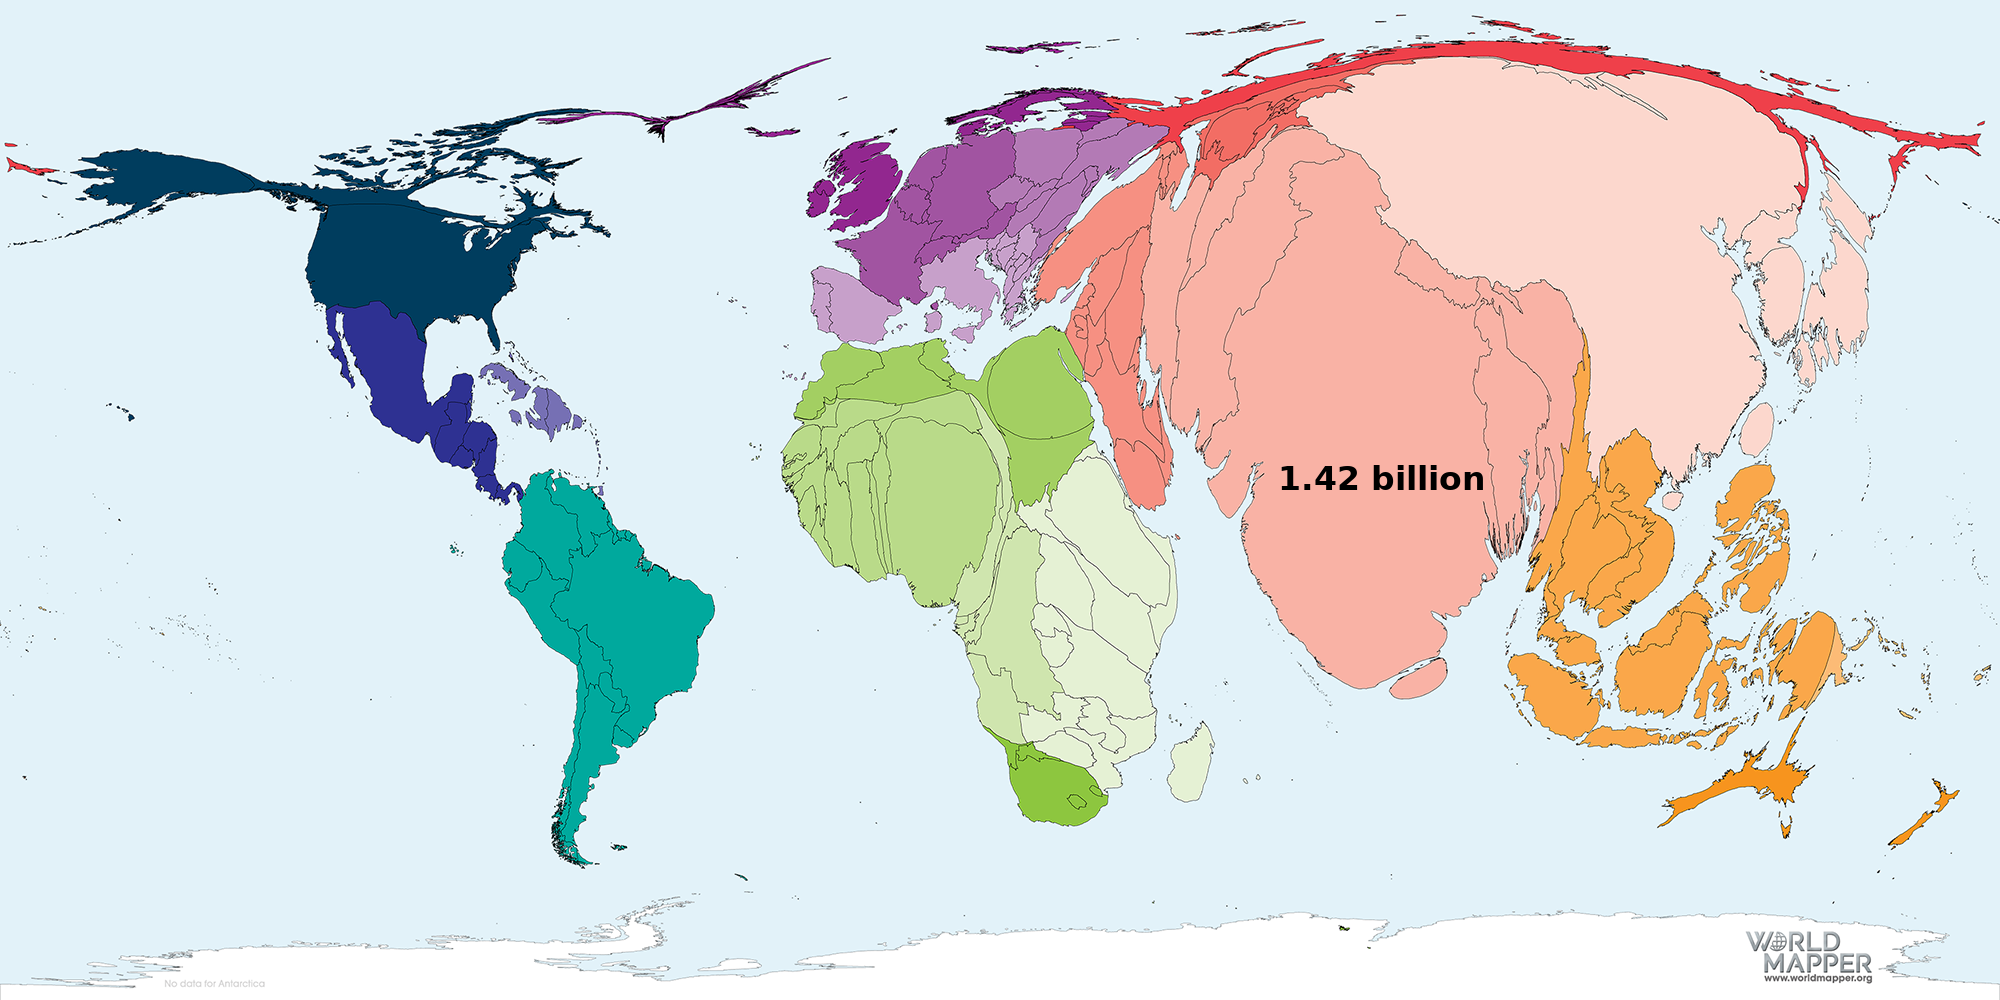
\includegraphics[width=0.6\paperwidth]{maps/population.png}

      \onslide<2->{population}
   \end{center}
\end{frame}

\begin{frame}
    \large
    Example puzzle 1. What links
          \begin{center}
                  magic, hugo, alfa, california
          \end{center}
   \onslide<2->{\textit{They all combine with a word from the NATO alphabet: Magic Mike, Victor Hugo, Alfa Romeo, and Hotel California}}
\end{frame}

\begin{frame}
   \large
   Example puzzle 2. What links
   \begin{center}
      \begin{minipage}{0.6\textwidth}
          \textit{%
              pe (skateboarding) \onslide<3->{= half-pi\textbf{pe}} \\
              thon (athletics) \onslide<4->{= half mara\textbf{thon}} \\
              son (wrestling) \onslide<5->{= half nel\textbf{son}} \\
              ley (tennis) \onslide<6->{= half-vol\textbf{ley}}}%
      \end{minipage}
   \end{center}

   \onslide<2->{Halves}%

\end{frame}

\begin{frame}
\begin{center}
\Huge
Round 1: Switzerland
\end{center}
\end{frame}
\begin{frame}
\begin{center}
\Large
1. The current Swiss banknotes each correspond to a different theme. List the four themes of the 10, 20, 50, and 100 franc notes.
\end{center}
\end{frame}
\begin{frame}
\begin{center}
\Large
2. The earliest evidence of skiing comes from which modern-day country?
\\
\vspace{0.5em}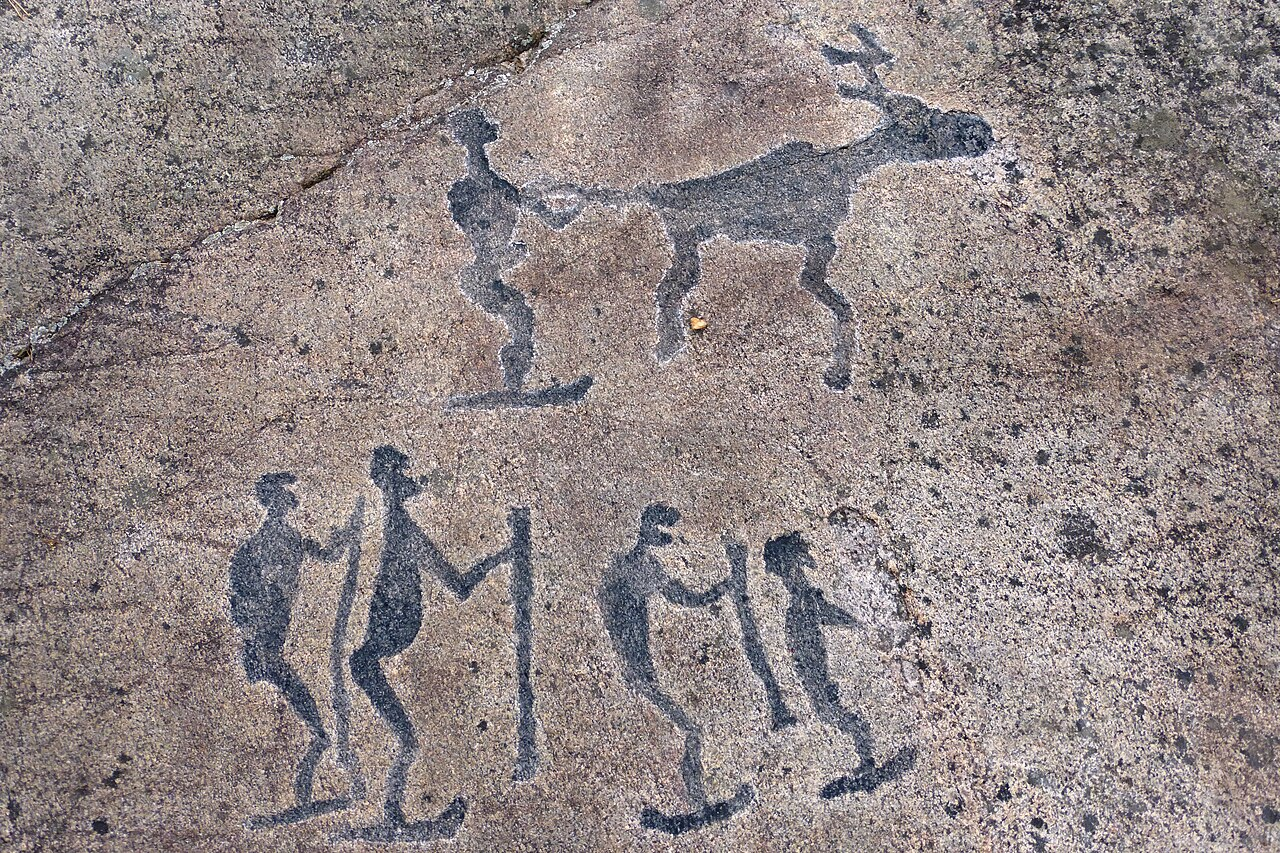
\includegraphics[height=0.6\paperheight]{images/skiing.jpg}
\end{center}
\end{frame}
\begin{frame}
\begin{center}
\Large
3. Which romance from 2000 saw Johnny Depp star as the love interest of Juliette Binoche?
\end{center}
\end{frame}
\begin{frame}
\begin{center}
\Large
4. \Large Here is a sorted list of fruit. What metric have I used to rank them?
\begin{enumerate}
   \item avocado
   \item watermelon
   \item banana
   \item nectarines
   \item strawberries
\end{enumerate}

\end{center}
\end{frame}
\begin{frame}
\begin{center}
\Large
5. This is an emblem of which organisation?
\\
\vspace{0.5em}
\includegraphics[height=0.6\paperheight]{images/red_crystal.png}
\end{center}
\end{frame}
\begin{frame}
\begin{center}
\Large
6. In ``A Grand Day Out'', why do Wallace and Gromit go to the moon?
\end{center}
\end{frame}
\begin{frame}
\begin{center}
\Large
7. What object has a face, a crown, and a lug?
\end{center}
\end{frame}
\begin{frame}
8. Which of the following is NOT a Swiss tradition?   
\begin{itemize}
      \item cow-vs-cow fighting
      \item burning a snowman
      \item men dressing up as bushes
      \item a sport that's a cross between golf and baseball
      \item a turnip parade
      \item wrapping women in quilts
   \end{itemize}

\end{frame}
\begin{frame}
\begin{center}
\Huge
Answers
\end{center}
\end{frame}
\begin{frame}
\begin{center}
\Large
1. The current Swiss banknotes each correspond to a different theme. List the four themes of the 10, 20, 50, and 100 franc notes.
\\
\onslide<2->{\vspace{1em}\textit{\begin{tabular}{cccccccc}
      \onslide<2->{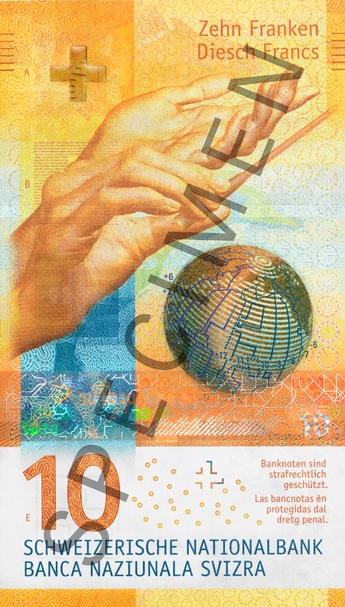
\includegraphics[width=0.1\textwidth]{images/CHF_10_9_front.jpg}} &
      \onslide<2->{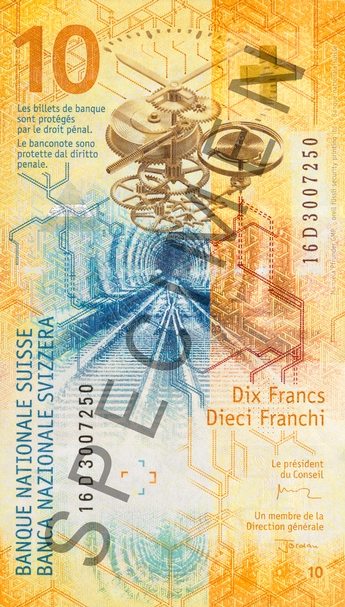
\includegraphics[width=0.1\textwidth]{images/CHF_10_9_back.jpg}} &
      \onslide<3->{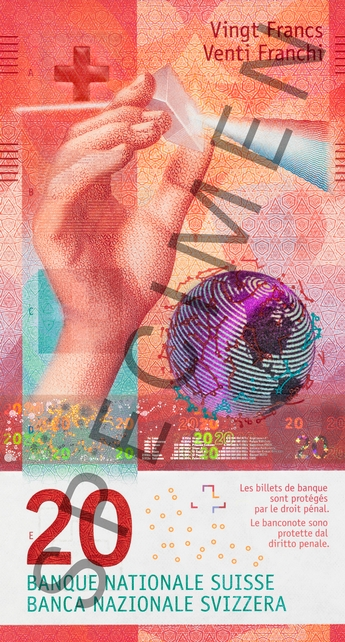
\includegraphics[width=0.1\textwidth]{images/CHF_20_9_front.jpg}} &
      \onslide<3->{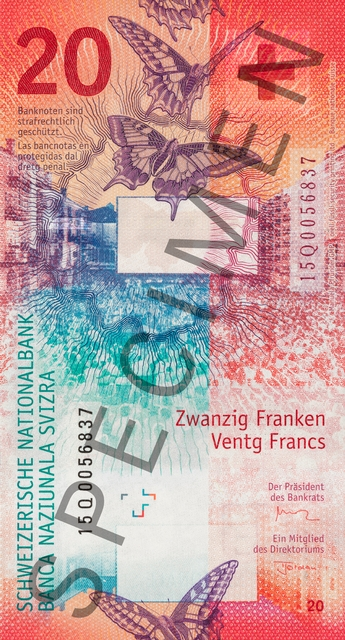
\includegraphics[width=0.1\textwidth]{images/CHF_20_9_back.jpg}} &
      \onslide<4->{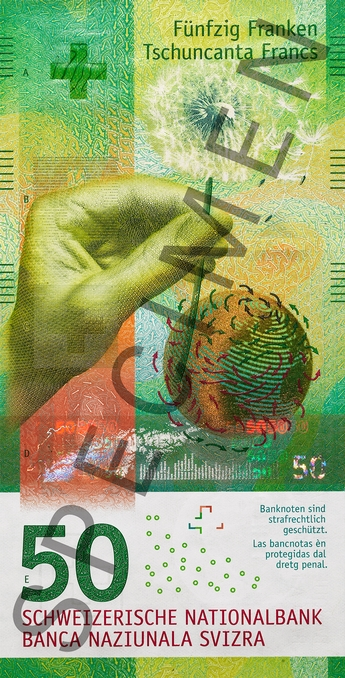
\includegraphics[width=0.1\textwidth]{images/CHF_50_9_front.jpg}} &
      \onslide<4->{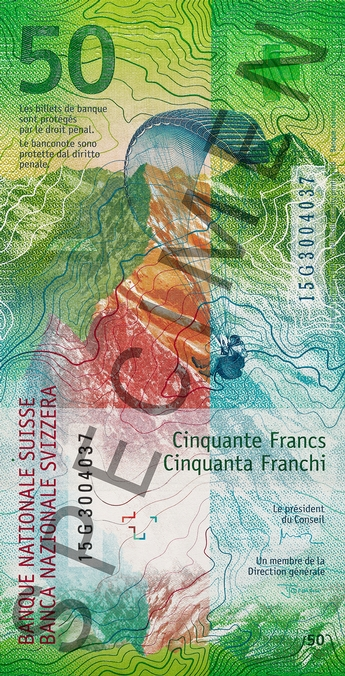
\includegraphics[width=0.1\textwidth]{images/CHF_50_9_back.jpg}} &
      \onslide<5->{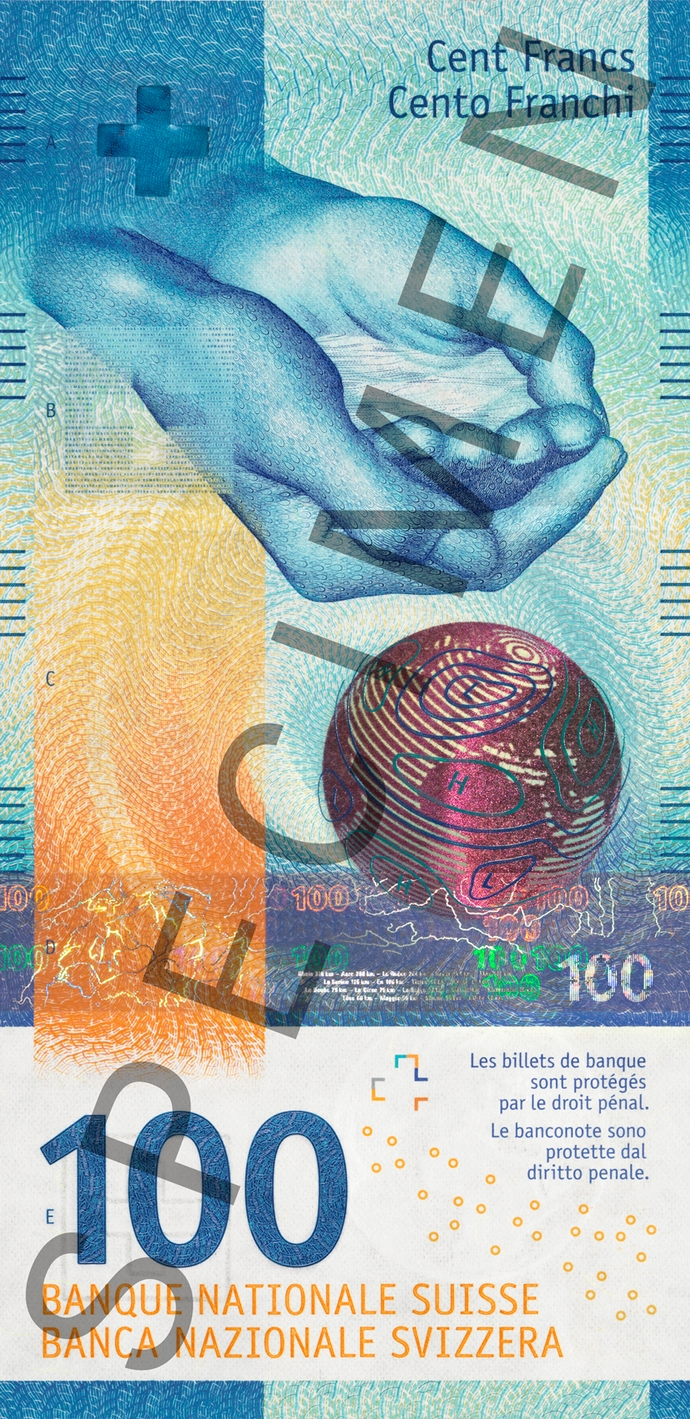
\includegraphics[width=0.1\textwidth]{images/CHF_100_9_front.jpg}} &
      \onslide<5->{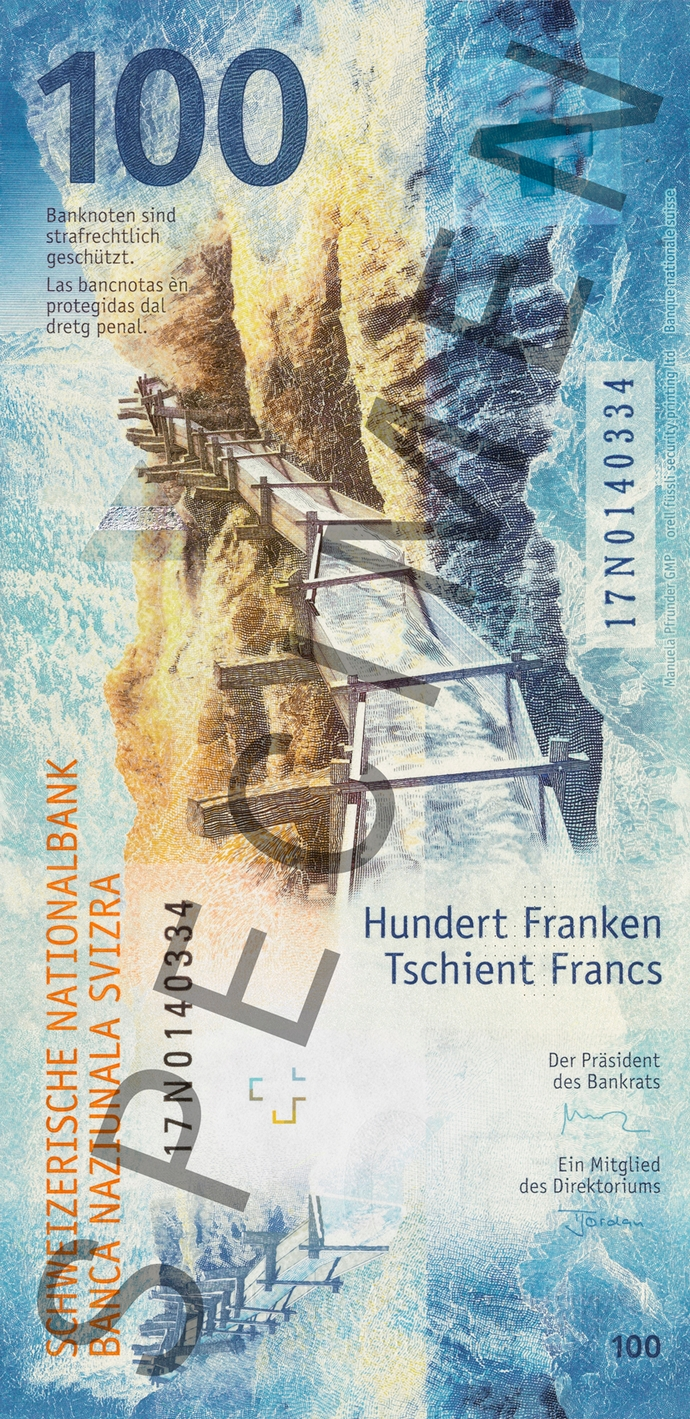
\includegraphics[width=0.1\textwidth]{images/CHF_100_9_back.jpg}} \\
      \multicolumn{2}{c}{\onslide<2->{\text{time}}} &
      \multicolumn{2}{c}{\onslide<3->{\text{light}}} &
      \multicolumn{2}{c}{\onslide<4->{\text{wind}}} &
      \multicolumn{2}{c}{\onslide<5->{\text{water}}}
\end{tabular}

\vspace{1em}

\onslide<6->{(order not important; half a point for three correct answers)}
}}
\end{center}
\end{frame}
\begin{frame}
\begin{center}
\Large
2. The earliest evidence of skiing comes from which modern-day country?
\\
\vspace{0.5em}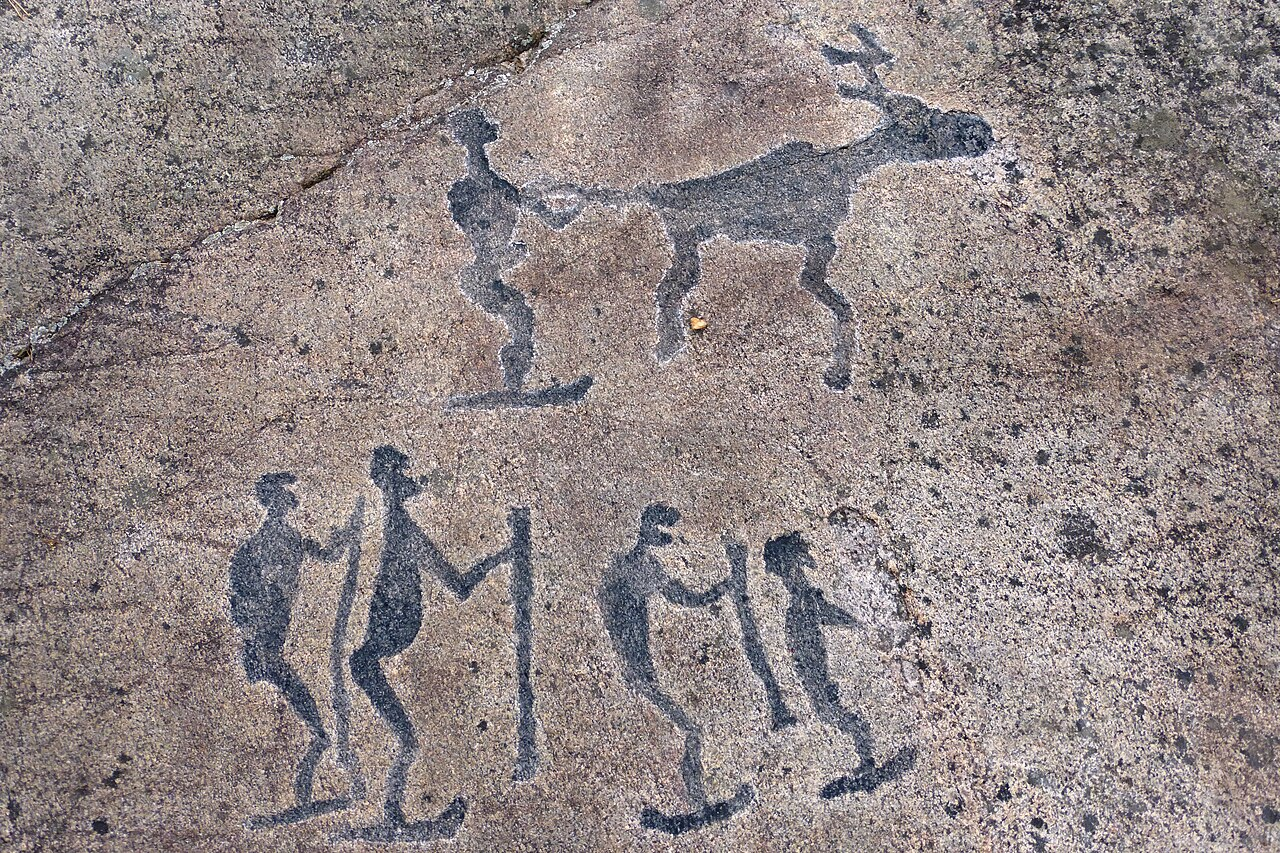
\includegraphics[height=0.6\paperheight]{images/skiing.jpg}
\\
\onslide<2->{\vspace{1em}\textit{Russia}}
\end{center}
\end{frame}
\begin{frame}
\begin{center}
\Large
3. Which romance from 2000 saw Johnny Depp star as the love interest of Juliette Binoche?
\\
\onslide<2>{\vspace{0.5em}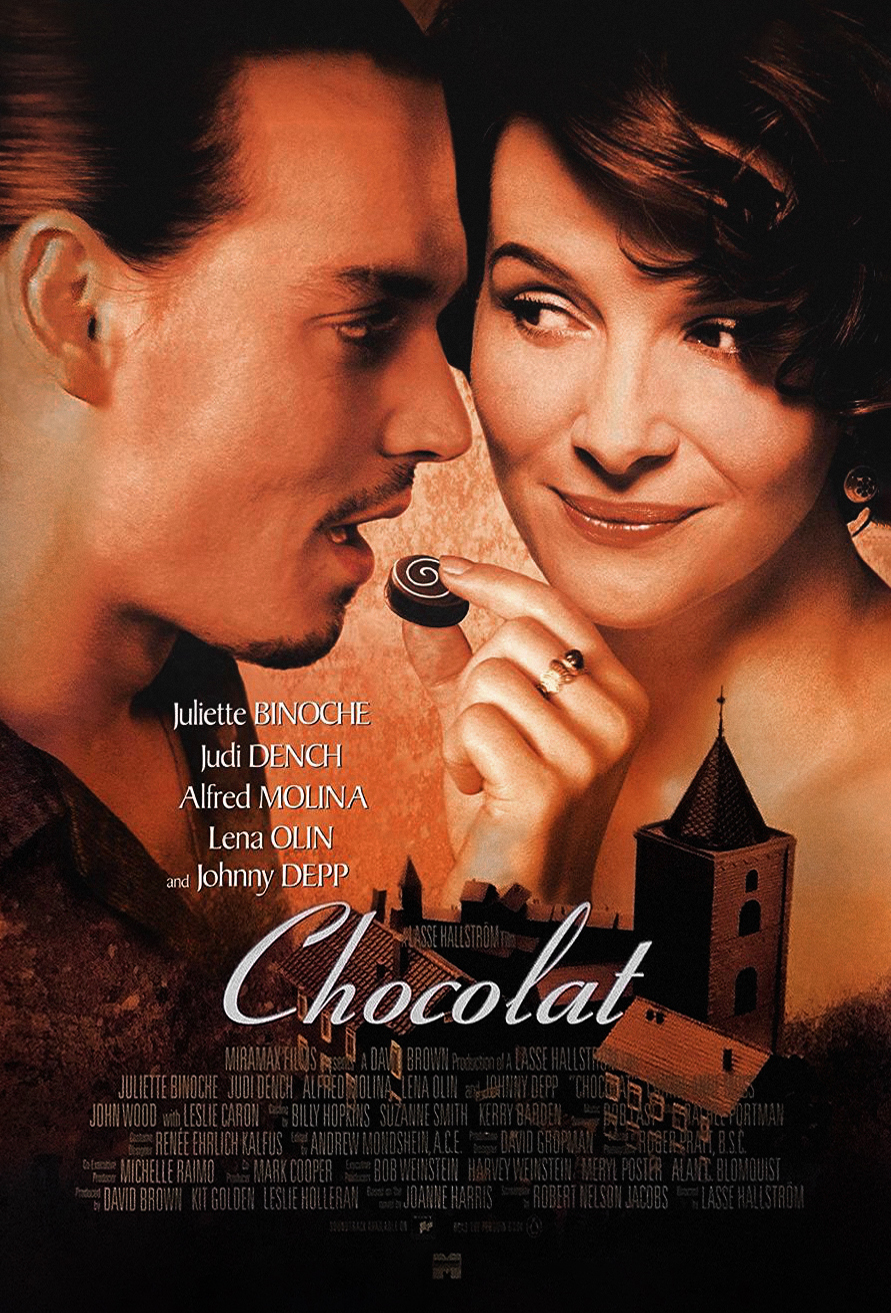
\includegraphics[height=0.6\paperheight]{images/chocolat.jpg}}
\\
\onslide<2->{\vspace{1em}\textit{Chocolat}}
\end{center}
\end{frame}
\begin{frame}
\Large 3. Here is a sorted list of fruit. What metric have I used to rank them?
\begin{enumerate}
   \item avocado \onslide<2->{6.3-6.6}
   \item watermelon \onslide<2->{5.2-5.6}
   \item banana \onslide<2->{4.5-5.2}
   \item nectarines \onslide<2->{3.9-4.2}
   \item strawberries \onslide<2->{3.0-3.9}
\end{enumerate}
\onslide<3->{\emph{ranked by neutrality}}

\end{frame}
\begin{frame}
\begin{center}
\Large
5. This is an emblem of which organisation?
\\
\only<1>{\vspace{0.5em}
\includegraphics[height=0.6\paperheight]{images/red_crystal.png}}
\only<2>{\vspace{0.5em}
\includegraphics[height=0.3\paperheight]{images/red_cross_cresent_crystal.png}}
\\
\onslide<2->{\vspace{1em}\textit{The Red Cross -- the ``Red Crystal'' is an alternative emblem used in contexts when both the cross and cresent would be religiously insensitive}}
\end{center}
\end{frame}
\begin{frame}
\begin{center}
\Large
6. In ``A Grand Day Out'', why do Wallace and Gromit go to the moon?
\\
\onslide<2>{\vspace{0.5em}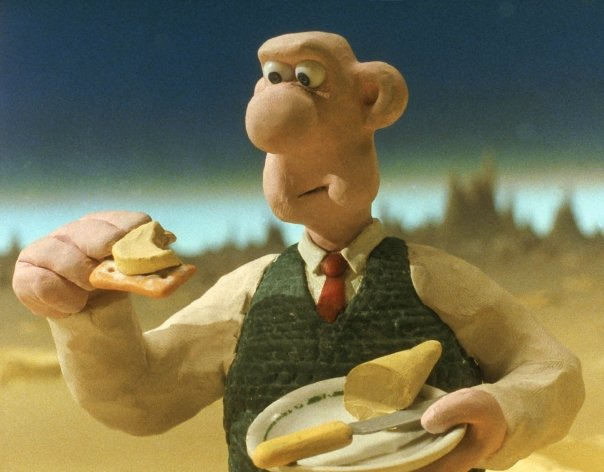
\includegraphics[height=0.6\paperheight]{images/grand_day_out.jpg}}
\\
\onslide<2->{\vspace{1em}\textit{to get some cheese}}
\end{center}
\end{frame}
\begin{frame}
\begin{center}
\Large
7. What object has a face, a crown, and a lug?
\\
\onslide<2>{\vspace{0.5em}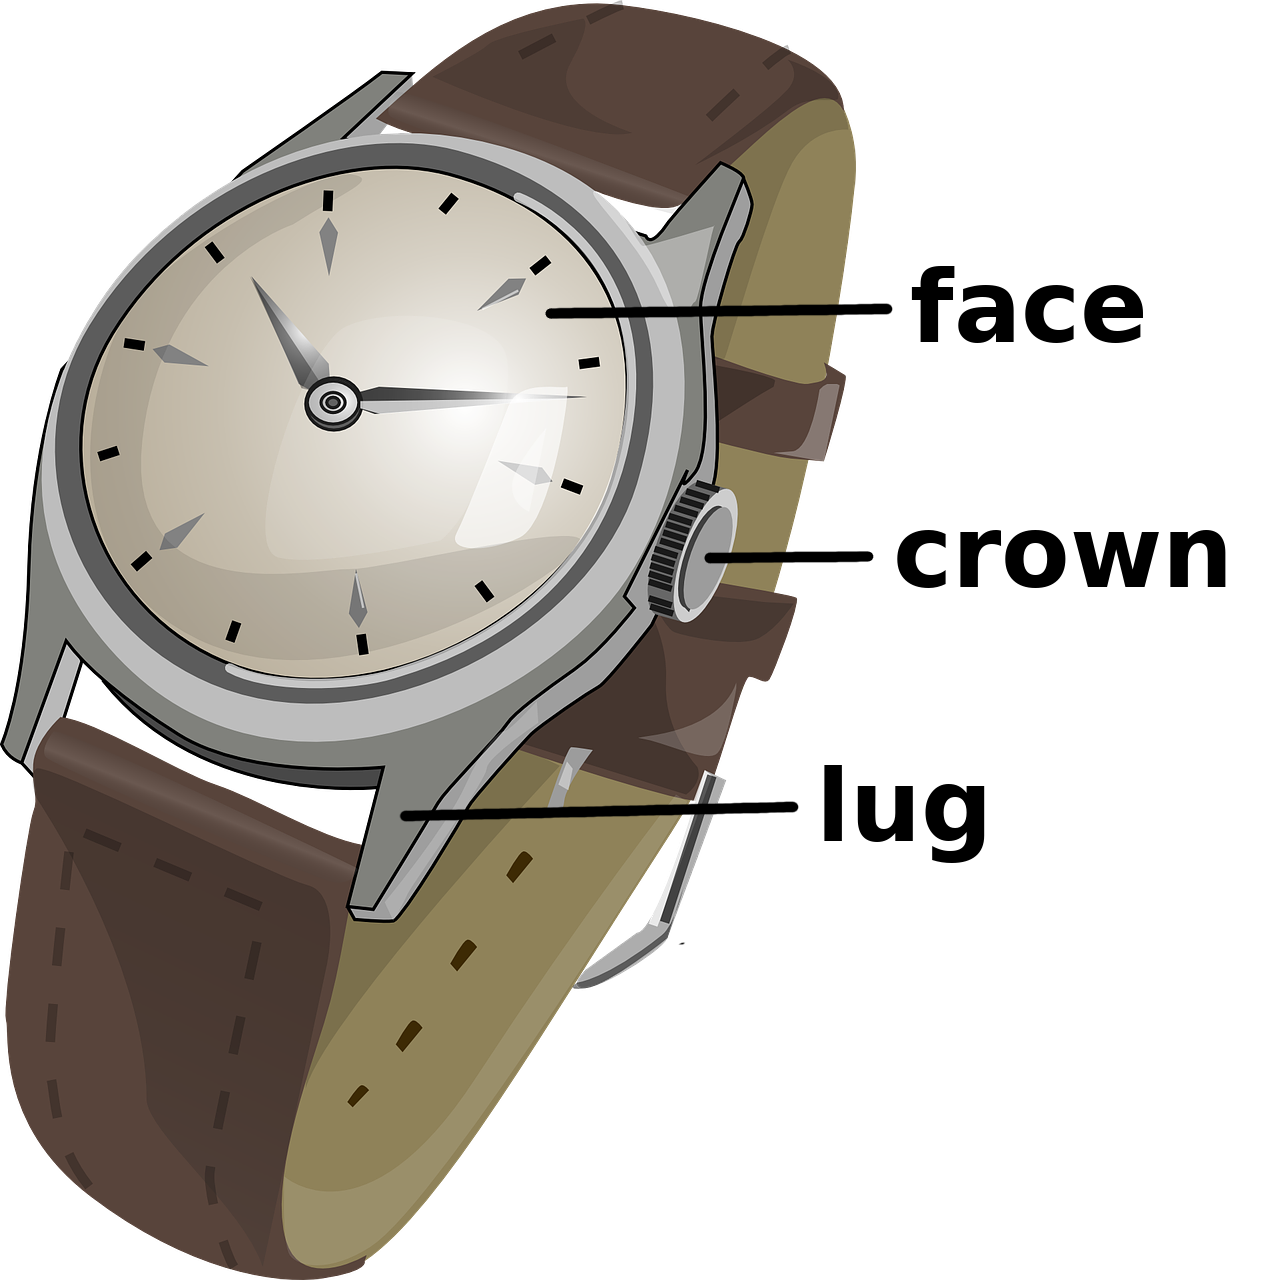
\includegraphics[height=0.6\paperheight]{images/watch.png}}
\\
\onslide<2->{\vspace{1em}\textit{a watch}}
\end{center}
\end{frame}
\begin{frame}
\begin{columns}
\begin{column}{0.5\paperwidth}
   8. Which of the following is NOT a Swiss tradition?   
\begin{itemize}
      \item cow-vs-cow fighting
      \item burning a snowman
      \item men dressing up as bushes
      \item a sport that's a cross between golf and baseball
      \item a turnip parade
      \item wrapping women in quilts
   \end{itemize}

\end{column}
\begin{column}{0.4\paperwidth}
   \begin{overlayarea}{\columnwidth}{0.6\paperheight}
      \only<2>{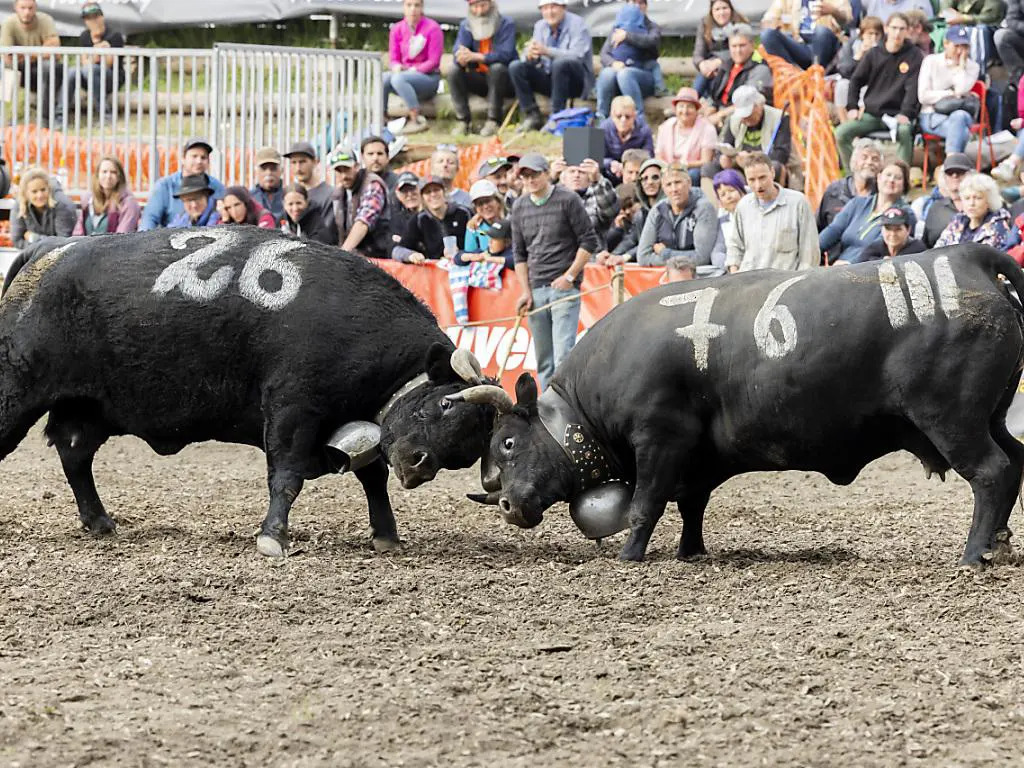
\includegraphics[width=\columnwidth]{images/cow_fighting.jpg}}
      \only<3>{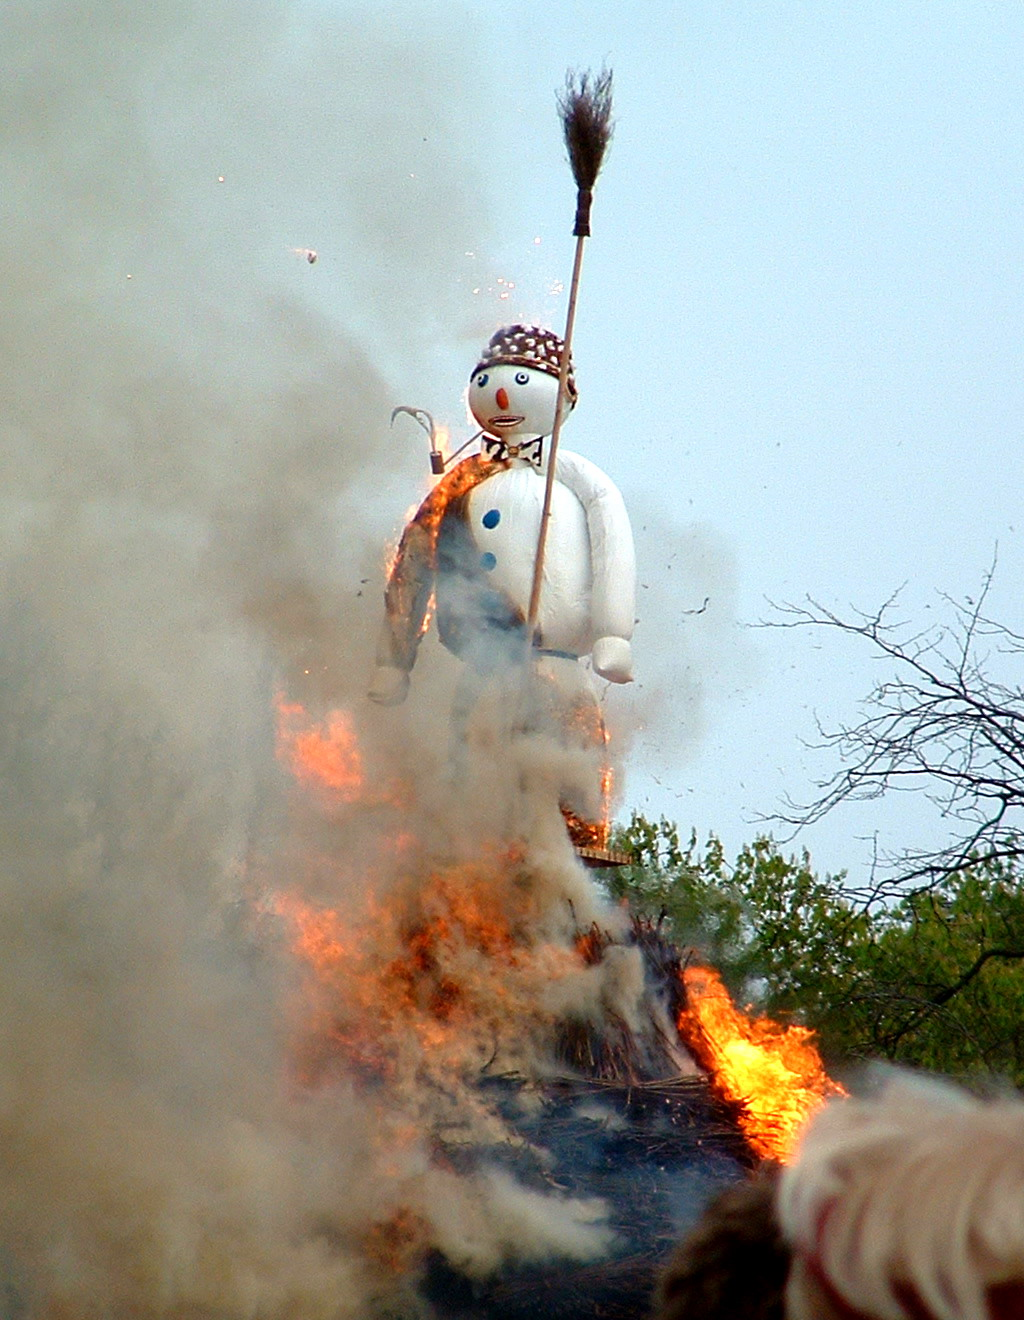
\includegraphics[height=0.6\paperheight]{images/boogg.jpg}}
      \only<4>{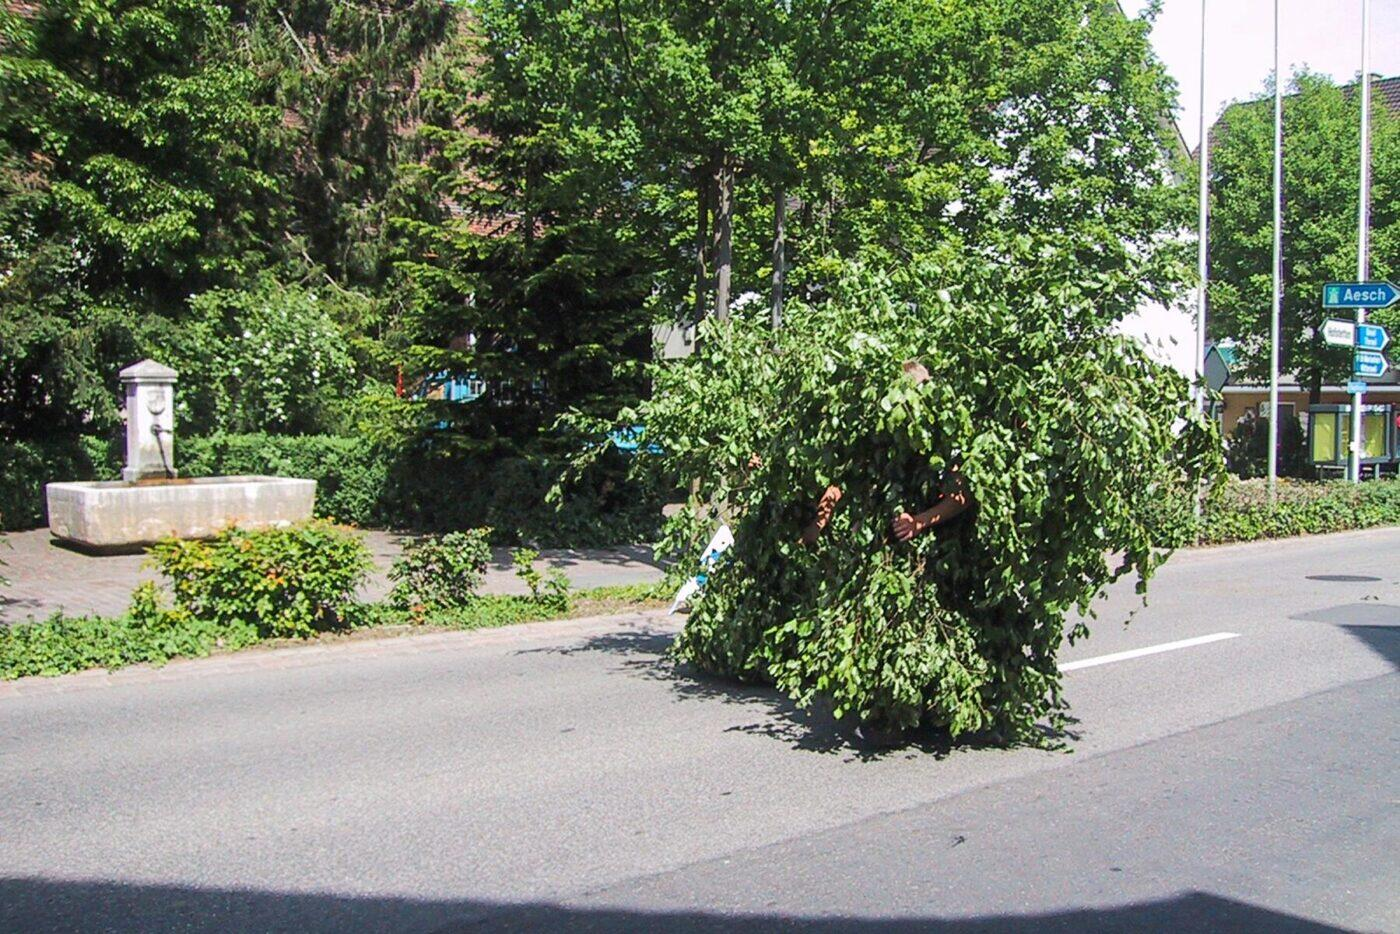
\includegraphics[width=\columnwidth]{images/bushes.jpg}}
      \only<5>{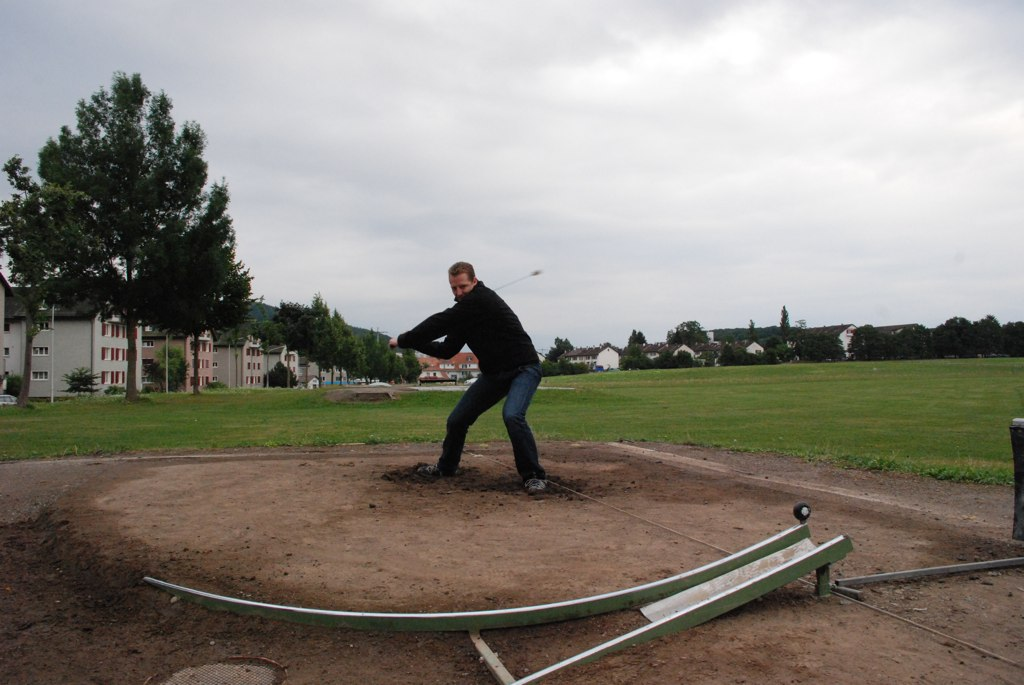
\includegraphics[width=\columnwidth]{images/Hornussen_Peschi.jpg}}
      \only<6>{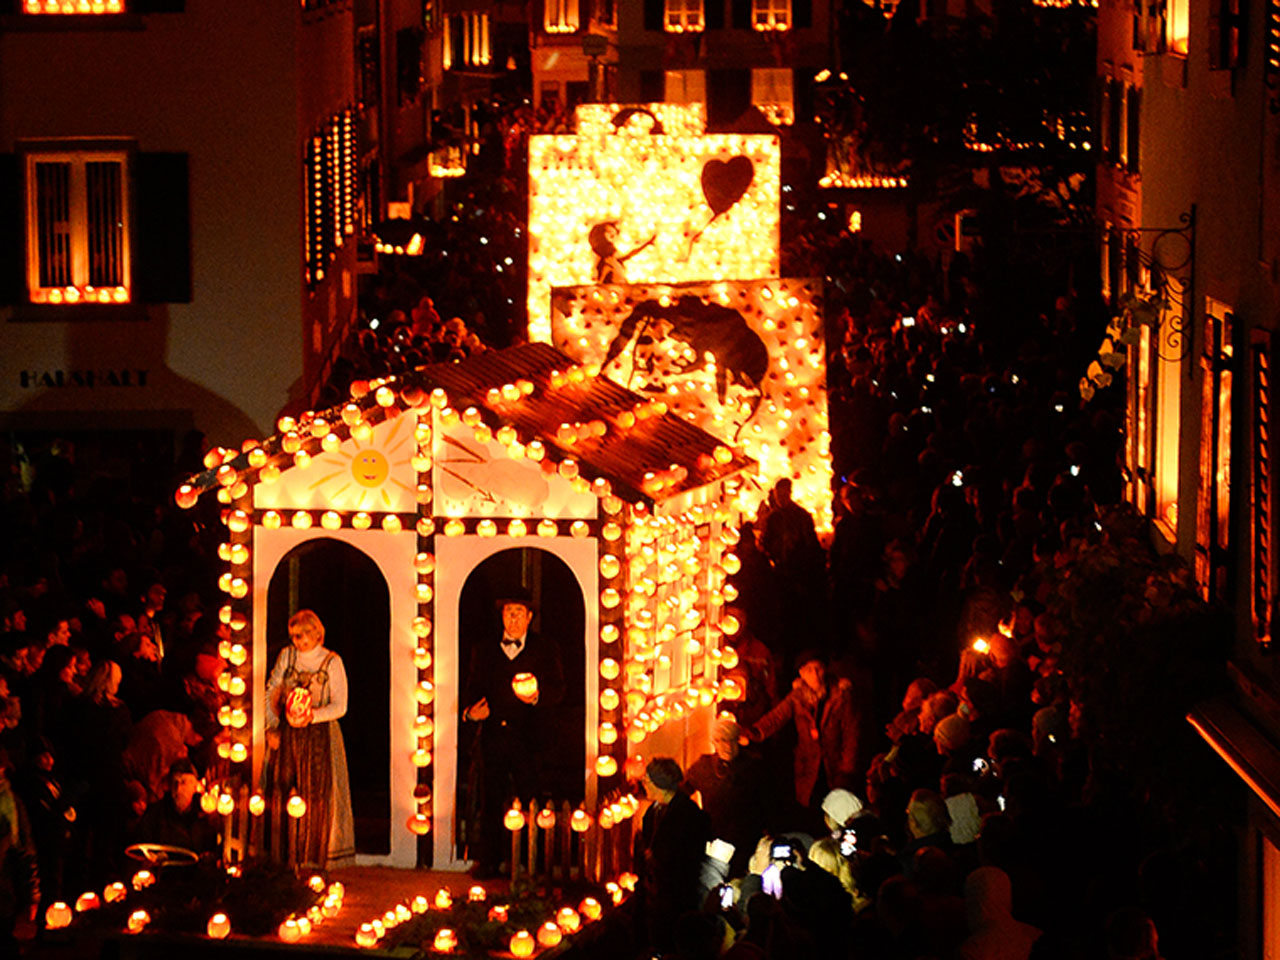
\includegraphics[width=\columnwidth]{images/turnip.jpg}}
   \end{overlayarea}
\end{column}
\end{columns}
\end{frame}
\begin{frame}
\begin{center}
\Huge
Round 2: ``Marvel''
\end{center}
\end{frame}
\begin{frame}
\begin{center}
\Large
1. Which popular hymn was written by a repentant ex-slave-ship owner?
\end{center}
\end{frame}
\begin{frame}
\begin{center}
\Large
2. Behind only Minecraft, what is the second-best selling video game of all time?
\end{center}
\end{frame}
\begin{frame}
\begin{center}
\Large
3. In tennis, what feat has only been achieved once, by Steffi Graf in 1988? (Here I am excluding wheelchair disciplines)
\end{center}
\end{frame}
\begin{frame}
\begin{center}
\Large
4. Which US National Park is this?
\\
\vspace{0.5em}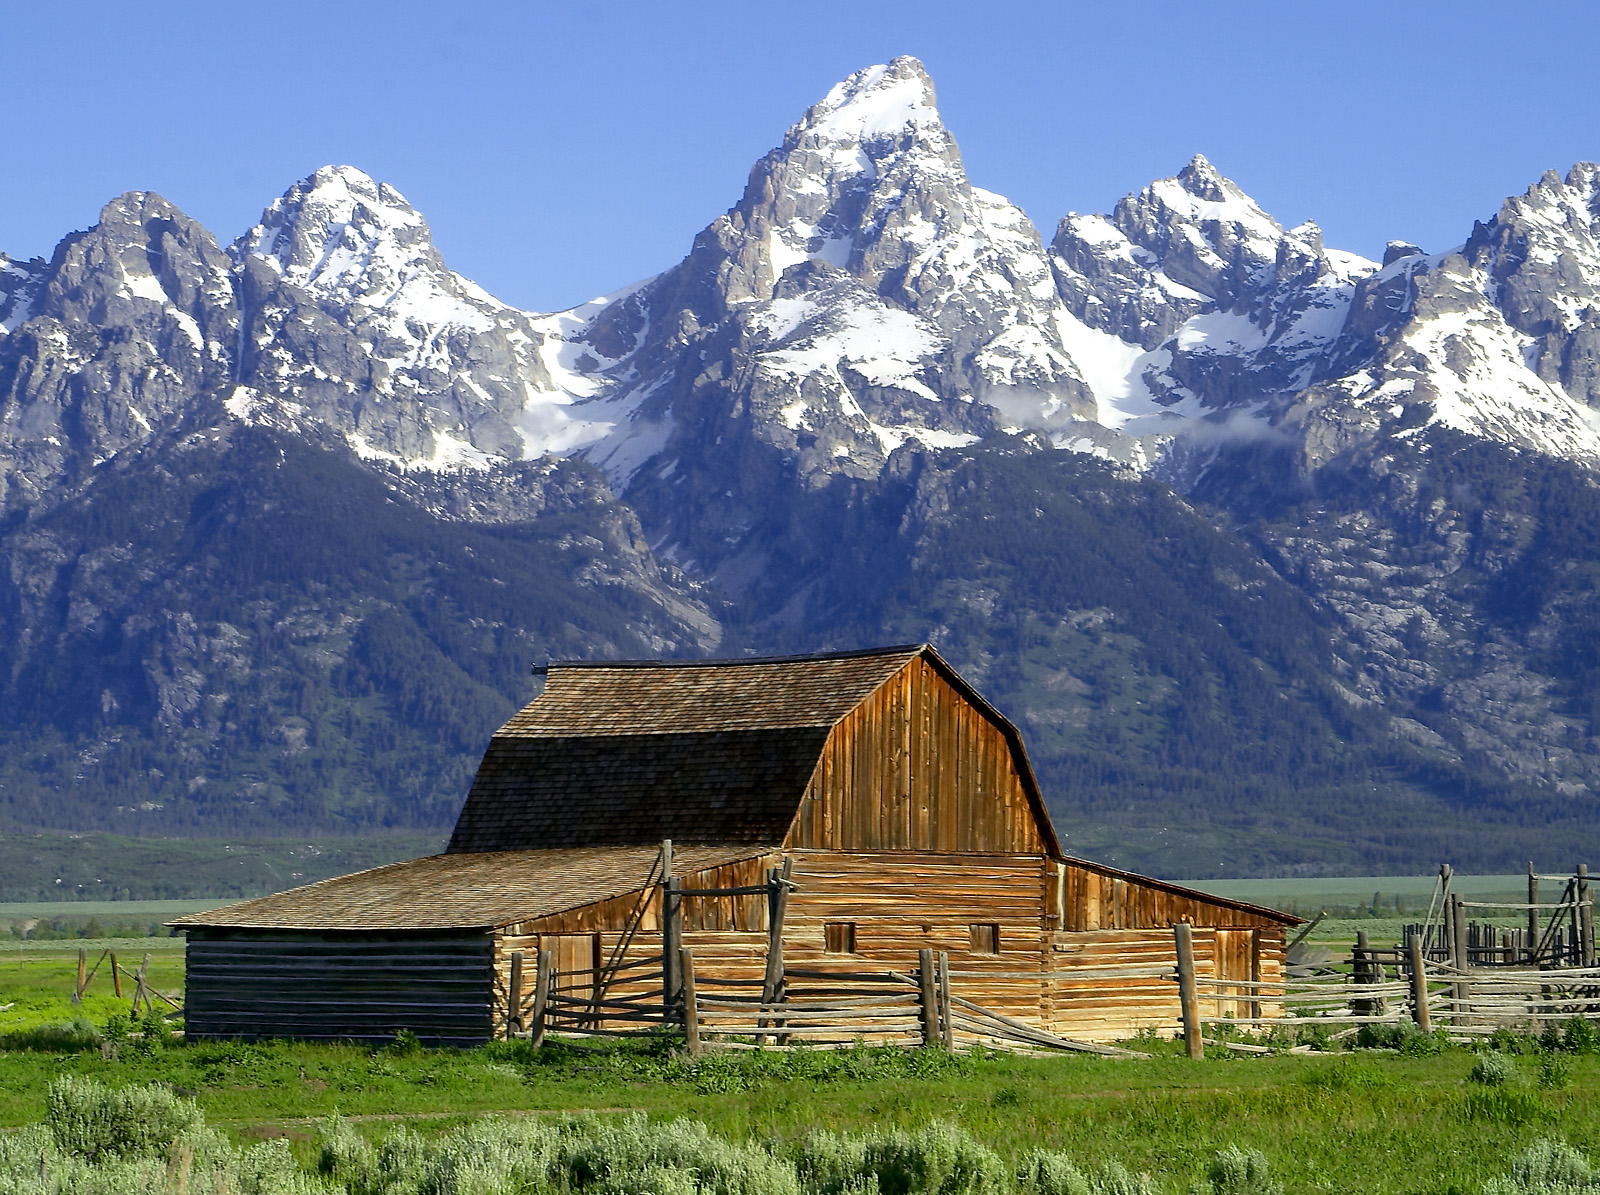
\includegraphics[height=0.6\paperheight]{images/grand_tetons.jpg}
\end{center}
\end{frame}
\begin{frame}
\begin{center}
\Large
5. What is the name of this design principle?
\begin{center}
    \begin{minipage}{0.8\textwidth}
        \begin{center}
        ``A software interface should behave in a way that most users will expect it to behave''
        \end{center}
    \end{minipage}
\end{center}

\end{center}
\end{frame}
\begin{frame}
\begin{center}
\Large
6. What was the first song from the 1990s to reach a billion streams on Spotify?
\end{center}
\end{frame}
\begin{frame}
\begin{center}
\Large
7. Of all the MARVEL films, which has the lowest rating on Rotten Tomatoes? It was released in 2015.
\end{center}
\end{frame}
\begin{frame}
\begin{center}
\Large
8. Name the seven wonders of the ancient world
\end{center}
\end{frame}
\begin{frame}
\begin{center}
\Huge
Answers
\end{center}
\end{frame}
\begin{frame}
\begin{center}
\Large
1. Which popular hymn was written by a repentant ex-slave-ship owner?
\\
\onslide<2->{\vspace{1em}\textit{Amazing Grace}}
\end{center}
\end{frame}
\begin{frame}
\begin{center}
\Large
2. Behind only Minecraft, what is the second-best selling video game of all time?
\\
\onslide<2>{\vspace{0.5em}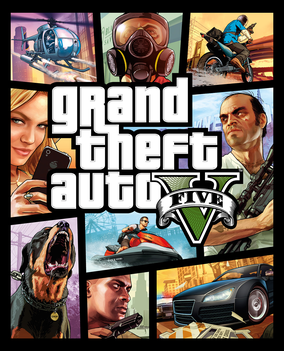
\includegraphics[height=0.6\paperheight]{images/gtav.png}}
\\
\onslide<2->{\vspace{1em}\textit{Grand Theft Auto V}}
\end{center}
\end{frame}
\begin{frame}
\begin{center}
\Large
3. In tennis, what feat has only been achieved once, by Steffi Graf in 1988? (Here I am excluding wheelchair disciplines)
\\
\onslide<2>{\vspace{0.5em}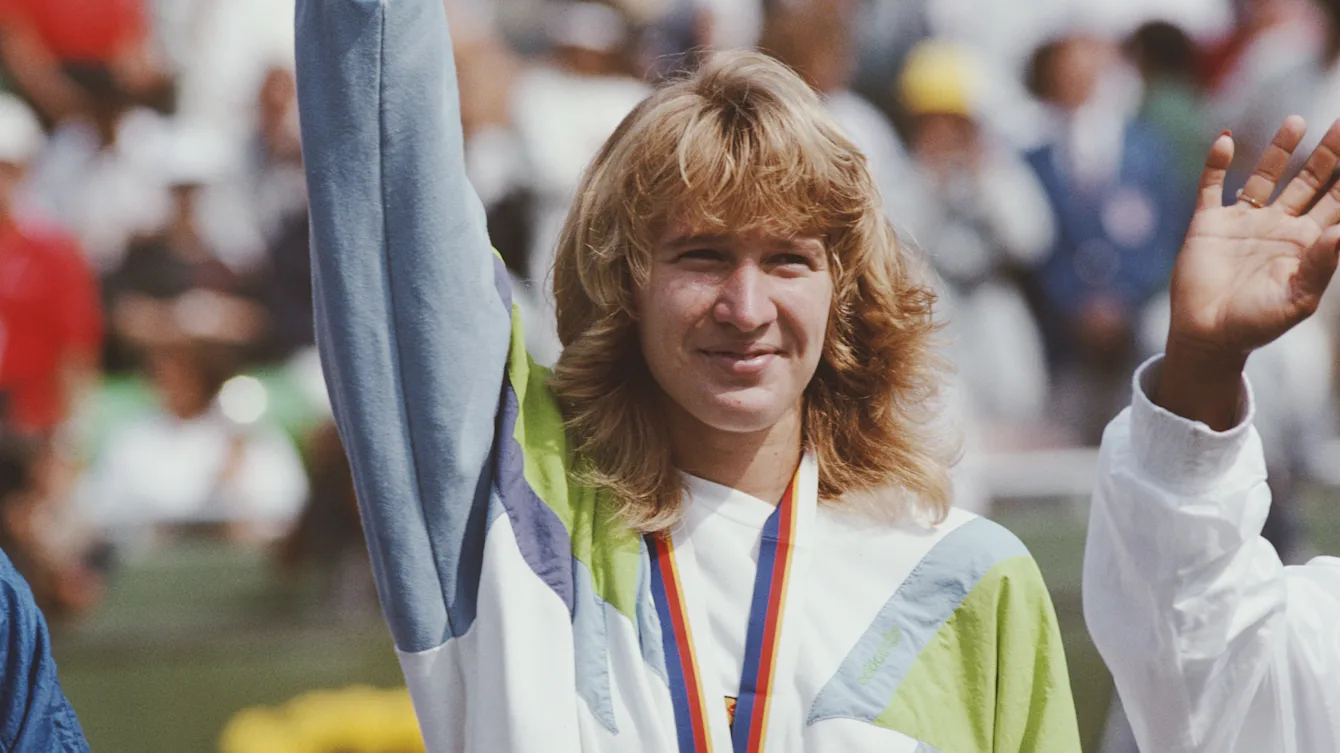
\includegraphics[height=0.6\paperheight]{images/steffi_graf.png}}
\\
\onslide<2->{\vspace{1em}\textit{a calendar Golden Grand Slam}}
\end{center}
\end{frame}
\begin{frame}
\begin{center}
\Large
4. Which US National Park is this?
\\
\vspace{0.5em}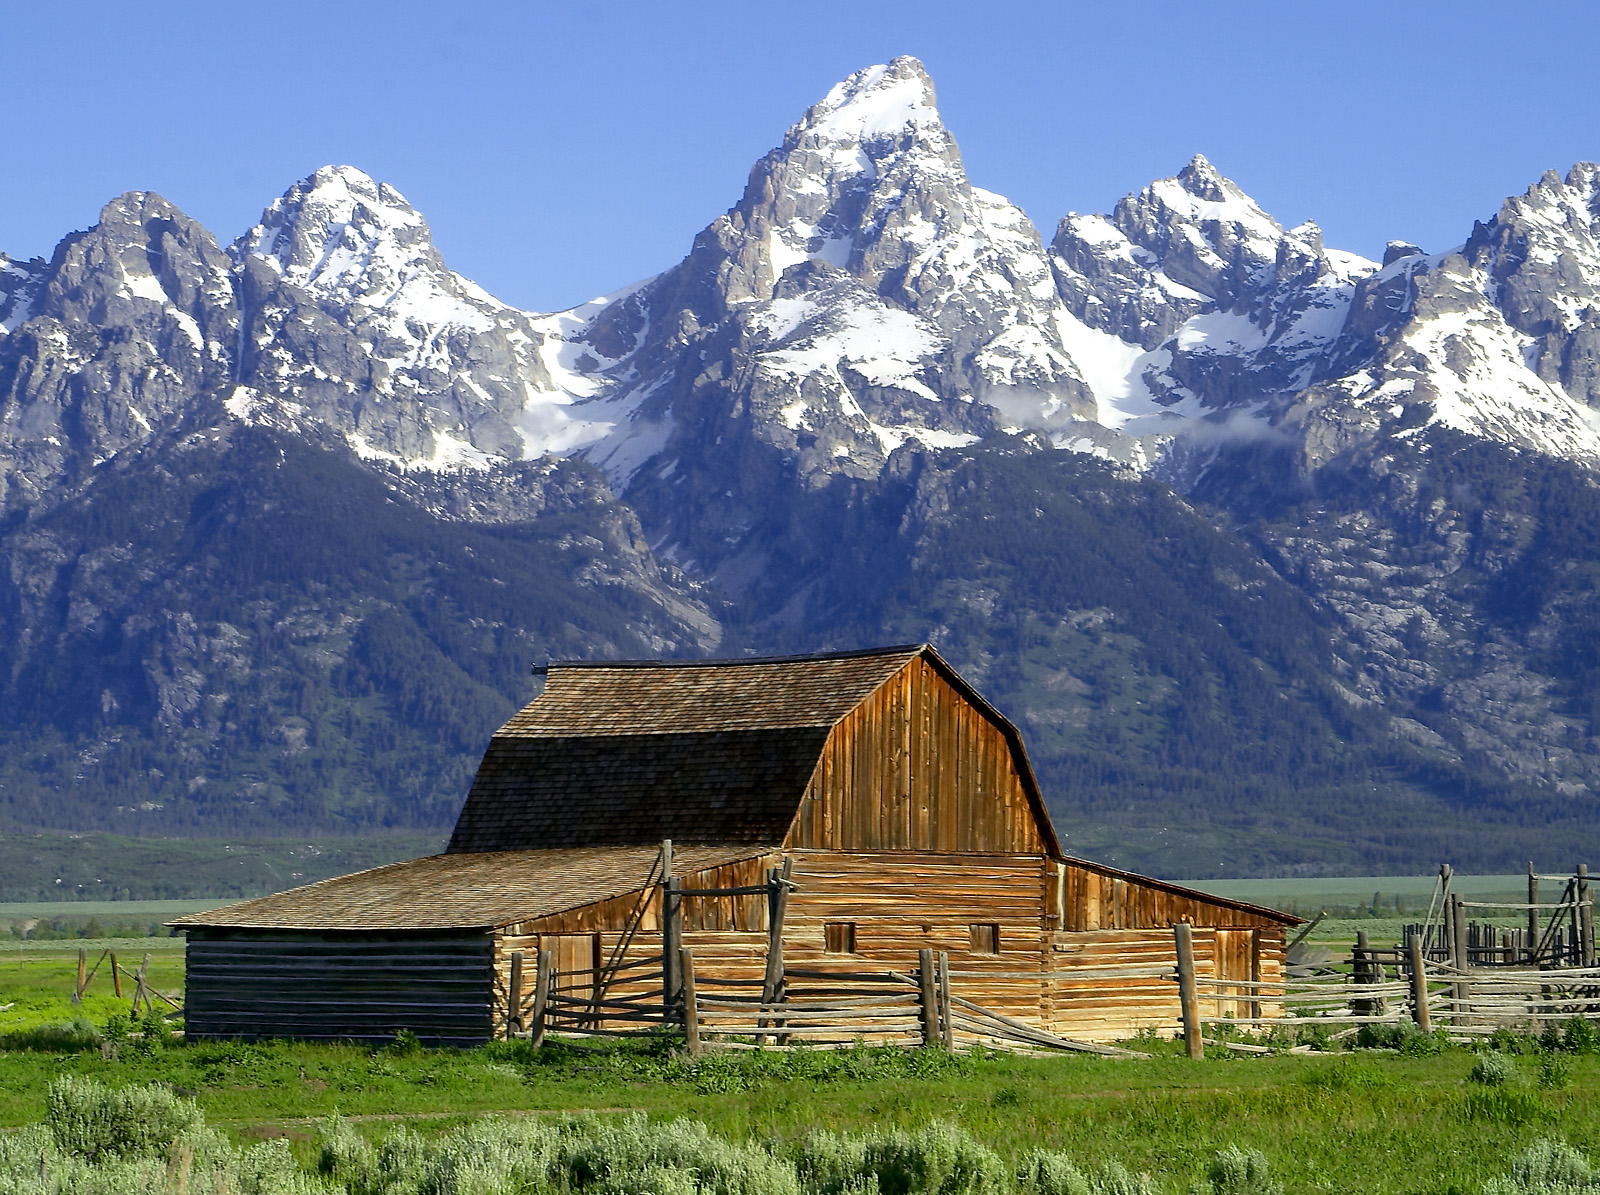
\includegraphics[height=0.6\paperheight]{images/grand_tetons.jpg}
\\
\onslide<2->{\vspace{1em}\textit{Grand Teton National Park}}
\end{center}
\end{frame}
\begin{frame}
\begin{center}
\Large
5. What is the name of this design principle?
\begin{center}
    \begin{minipage}{0.8\textwidth}
        \begin{center}
        ``A software interface should behave in a way that most users will expect it to behave''
        \end{center}
    \end{minipage}
\end{center}

\onslide<2->{\vspace{1em}\textit{the principle of least astonishment / surprise}}
\end{center}
\end{frame}
\begin{frame}
\begin{center}
\Large
6. What was the first song from the 1990s to reach a billion streams on Spotify?
\\
\onslide<2->{\vspace{1em}\textit{Wonderwall}}
\end{center}
\end{frame}
\begin{frame}
\begin{center}
\Large
7. Of all the MARVEL films, which has the lowest rating on Rotten Tomatoes? It was released in 2015.
\\
\onslide<2>{\vspace{0.5em}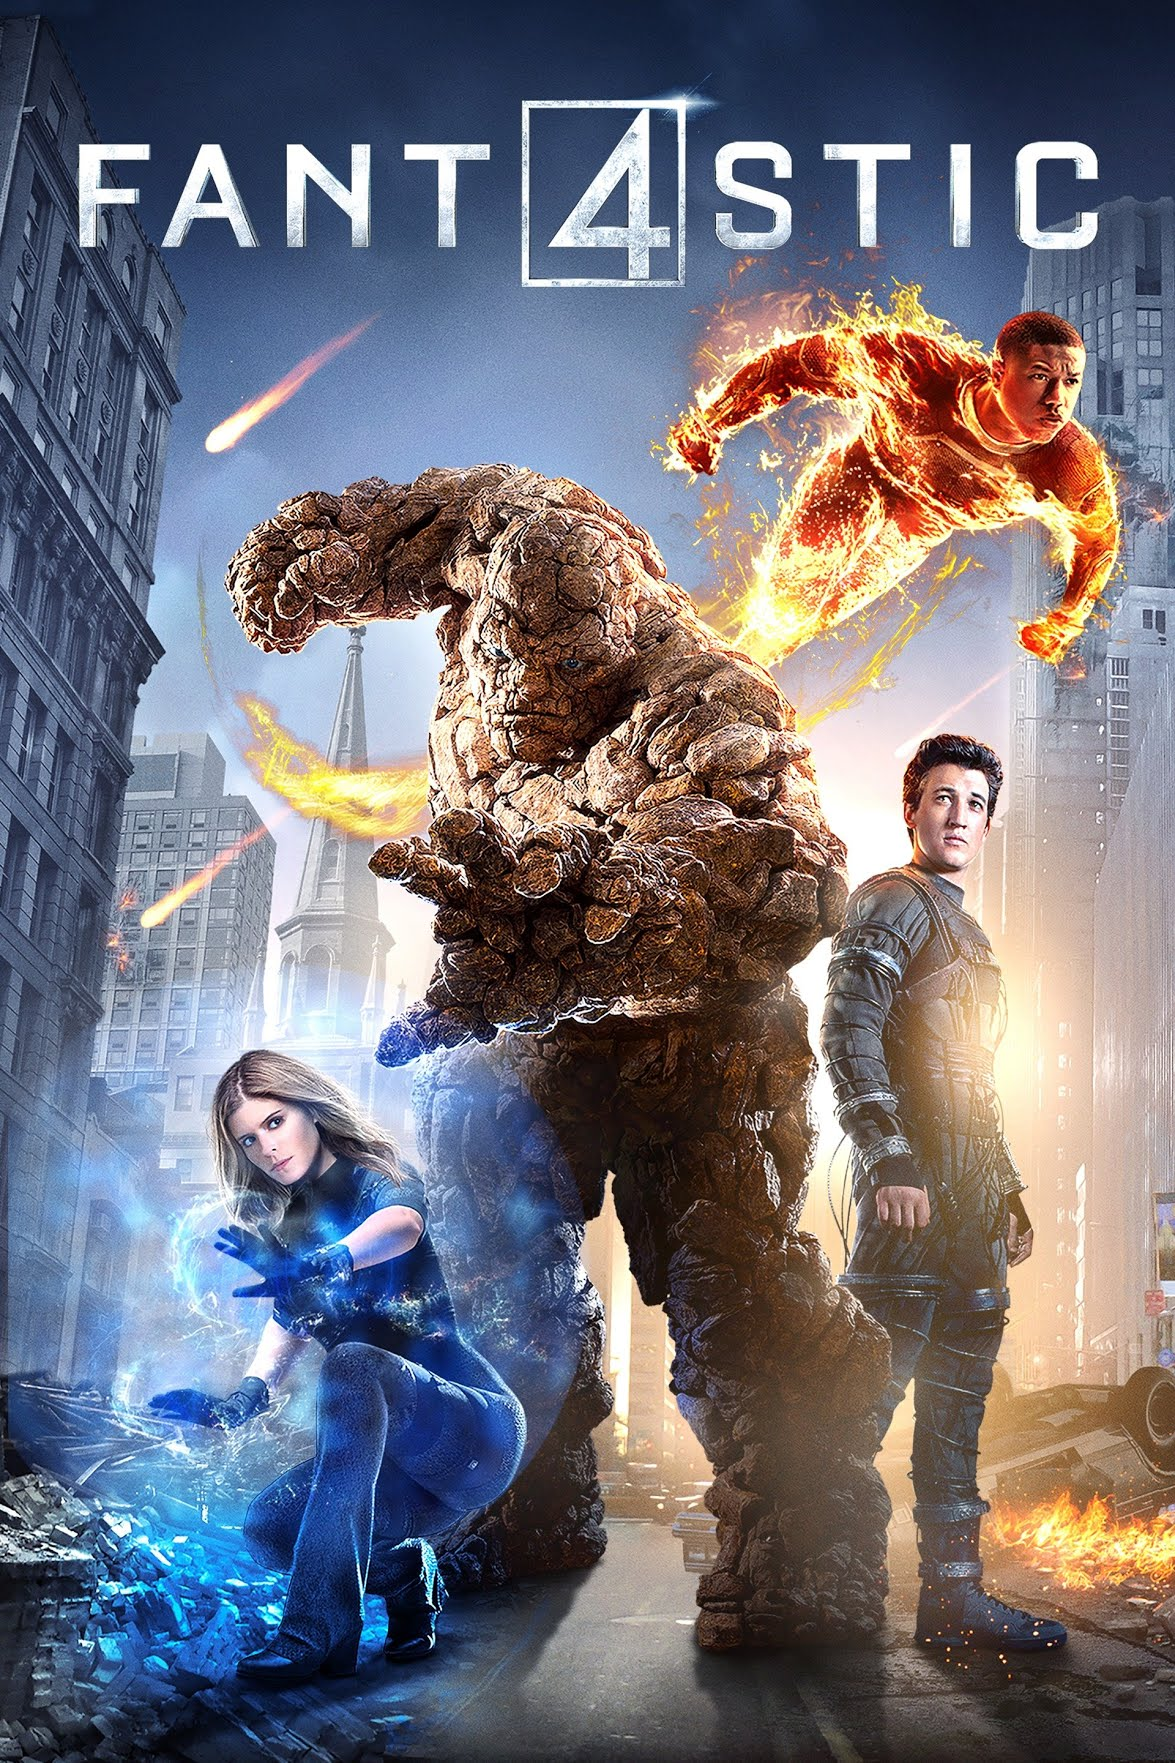
\includegraphics[height=0.6\paperheight]{images/fantastic_four.jpeg}}
\\
\onslide<2->{\vspace{1em}\textit{Fantastic Four (a measly 9\%)}}
\end{center}
\end{frame}
\begin{frame}
\begin{center}
\Large
8. Name the seven wonders of the ancient world
\\
\onslide<2->{\vspace{1em}\textit{The Colossus of Rhodes, the Great Pyramid of Giza, the Hanging Gardens of Babylon, the Statue of Zeus at Olympia, the Temple of Artemis at Ephesus, the Mausoleum at Halicarnassus, and the Lighthouse of Alexandria}}
\end{center}
\end{frame}
\begin{frame}
\begin{center}
\Huge
Round 3: Design and Discovery of Novel Materials
\end{center}
\end{frame}
\begin{frame}
\begin{center}
\Large
1. What is matter?
\\
\vspace{0.5em}
\includegraphics[height=0.25\paperheight]{images/matter.png}
\end{center}
\end{frame}
\begin{frame}
\begin{center}
\Large
2. ``Prophet Song'', ``The Seven Moons of Maali Almeida'', and ``The Promise'' are all prize-winning whats?
\end{center}
\end{frame}
\begin{frame}
\begin{center}
\Large
3. What car is this?
\blfootnote{photo credit: Wikimedia Commons}
\\
\vspace{0.5em}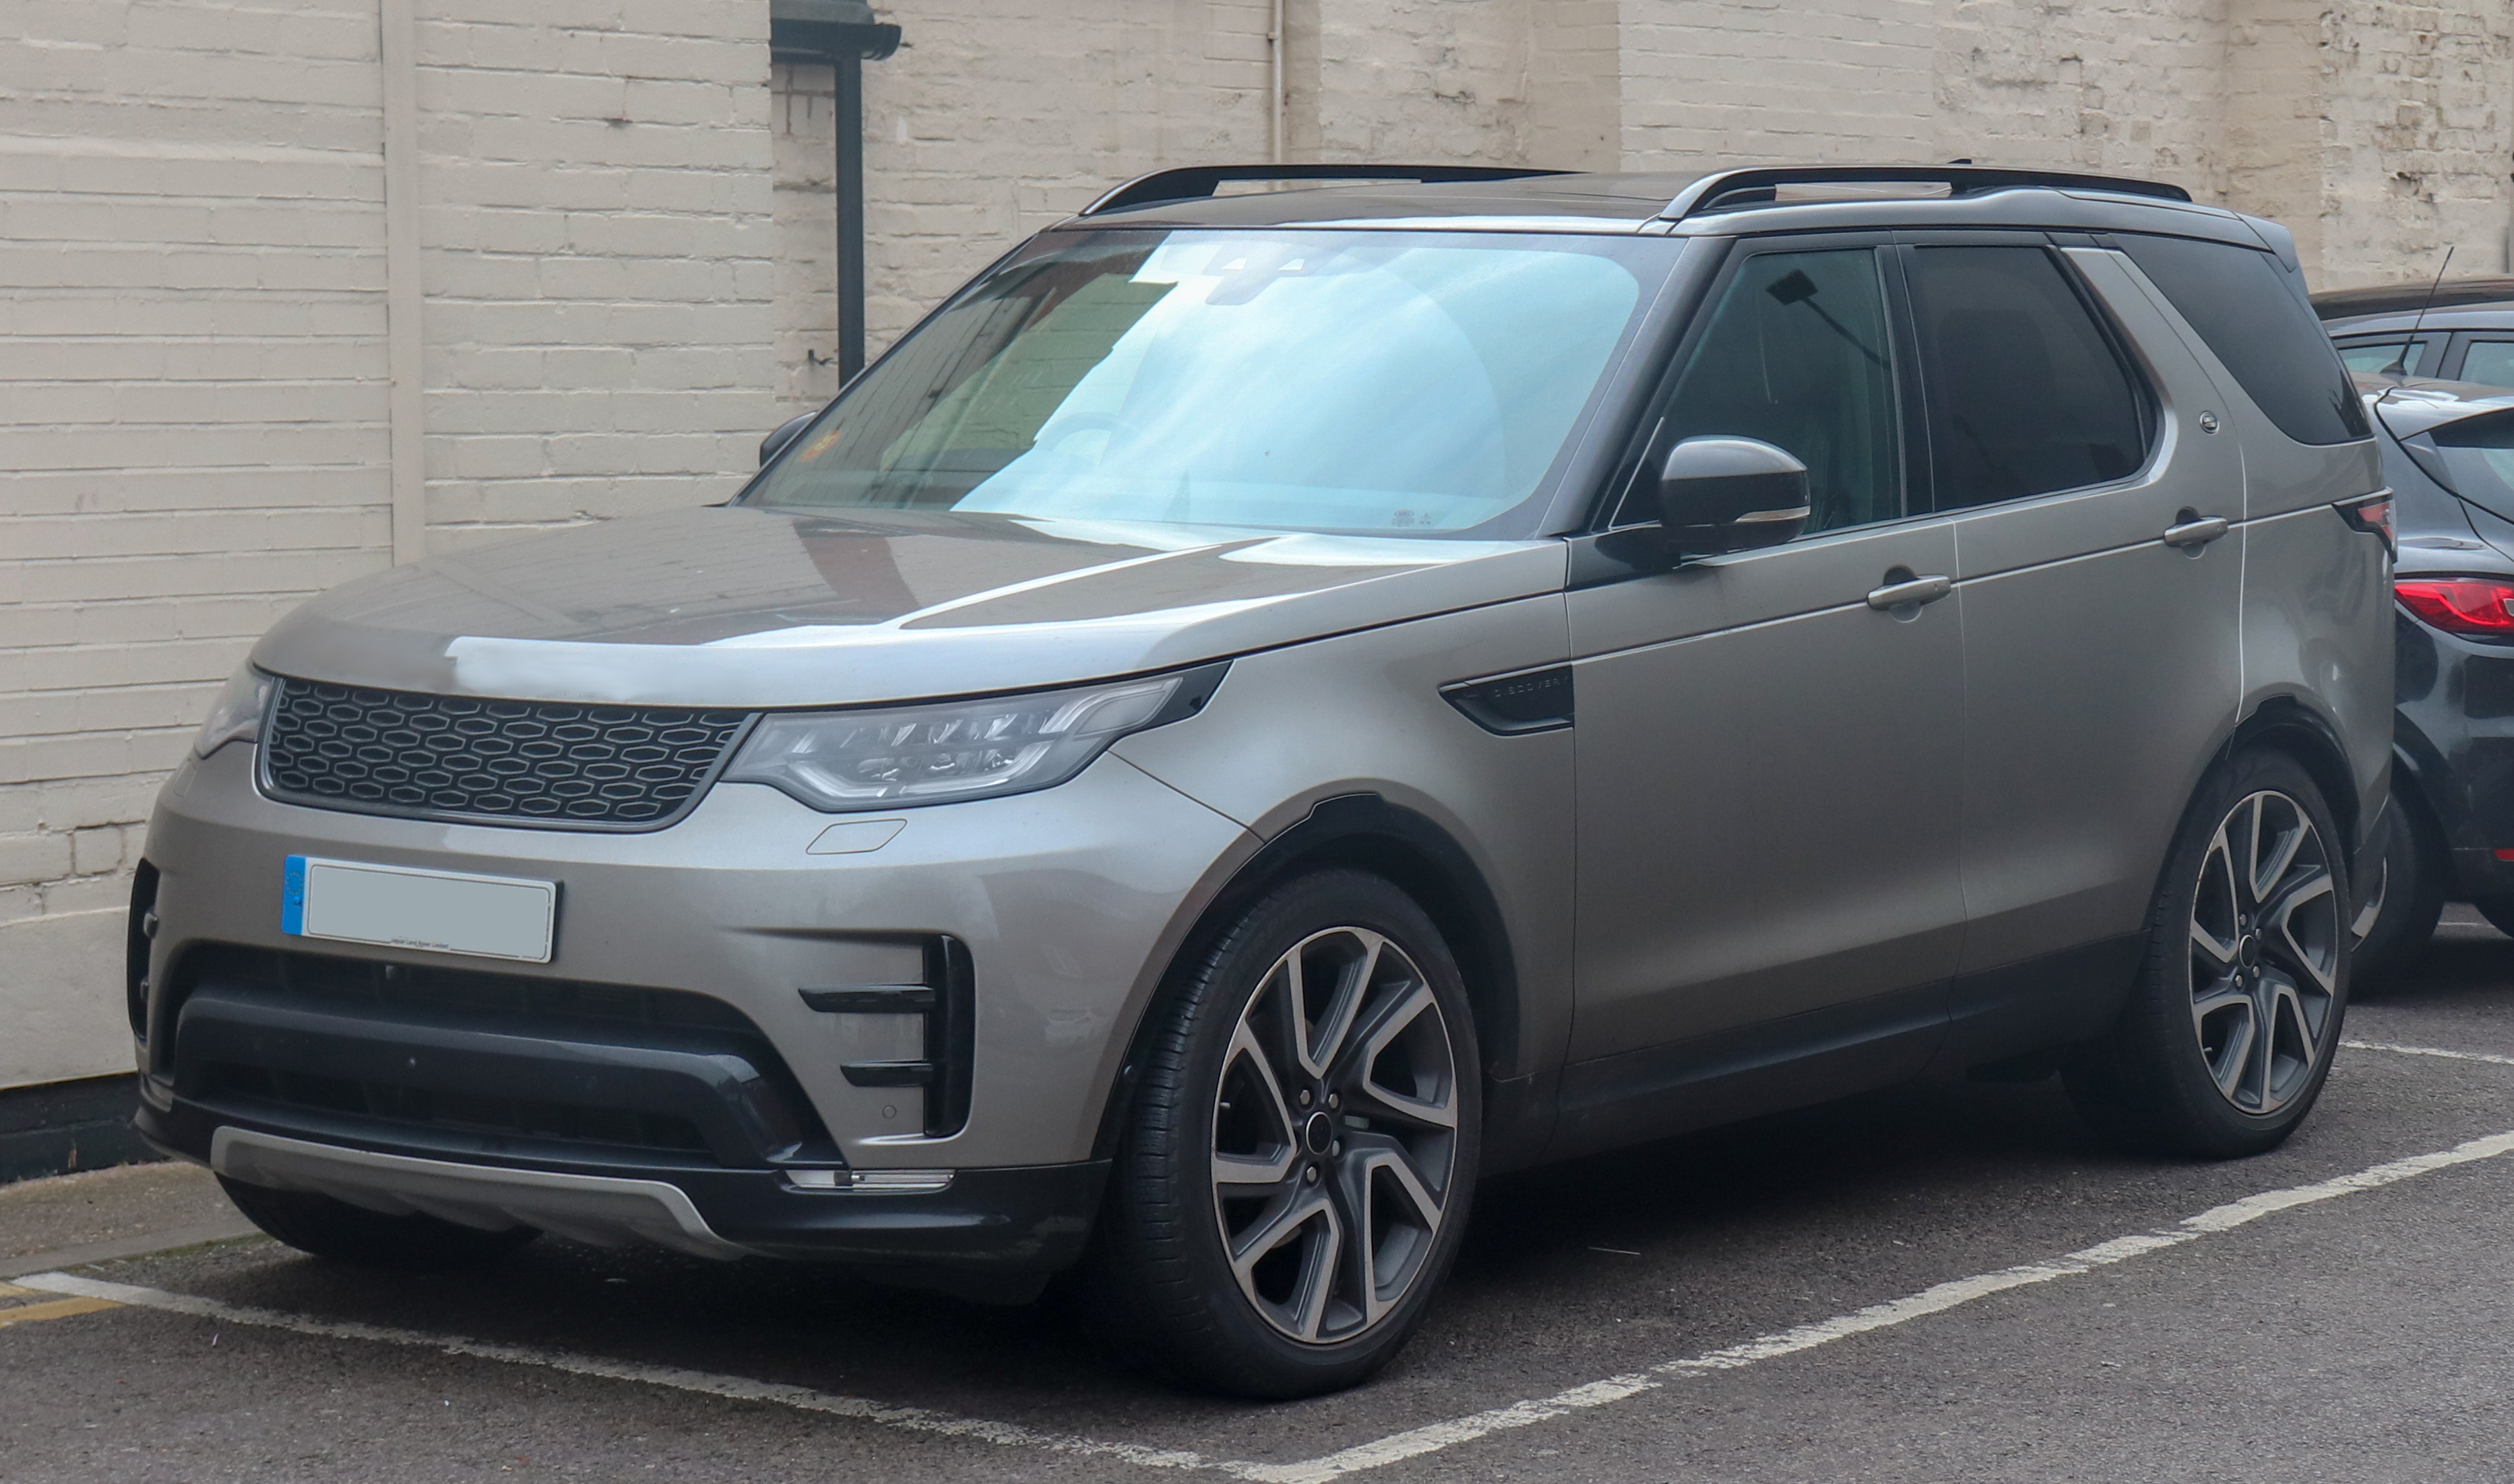
\includegraphics[height=0.6\paperheight]{images/land_rover_discovery.jpg}
\end{center}
\end{frame}
\begin{frame}
\begin{center}
\Large
4. gabardine, lawn, brocade, and french terry are all examples of what?
\end{center}
\end{frame}
\begin{frame}
\begin{center}
\Large
5. The Pritzker Prize is the most prestigious international prize in what field?
\end{center}
\end{frame}
\begin{frame}
\begin{center}
\Large
6. What parent company owns (among other things) DC Comics, HBO, CNN, and Eurosport?
\end{center}
\end{frame}
\begin{frame}
\begin{center}
\Large
7. ``Die Neue Sammlung'', in Munich, is the largest what in the world? (It translates to ``The New Collection'')
\end{center}
\end{frame}
\begin{frame}
\begin{center}
\Large
8. This is the opening verse to which song?
\begin{center}
    \begin{minipage}{0.6\textwidth}
        \textit{%
            Some boys kiss me \\
            Some boys hug me \\
            I think they're ok \\
            If they don't give me proper credit \\
            I just walk away}%
    \end{minipage}
\end{center}

\end{center}
\end{frame}
\begin{frame}
\begin{center}
\Huge
Answers
\end{center}
\end{frame}
\begin{frame}
\begin{center}
\Large
1. What is matter?
\\
\vspace{0.5em}
\includegraphics[height=0.25\paperheight]{images/matter.png}
\\
\onslide<2->{\vspace{1em}\textit{a connectivity standard for smart home and IoT devices}}
\end{center}
\end{frame}
\begin{frame}
\begin{center}
\Large
2. ``Prophet Song'', ``The Seven Moons of Maali Almeida'', and ``The Promise'' are all prize-winning whats?
\\
\onslide<2->{\vspace{1em}\textit{\begin{center}
\begin{tabular}{ccc}
   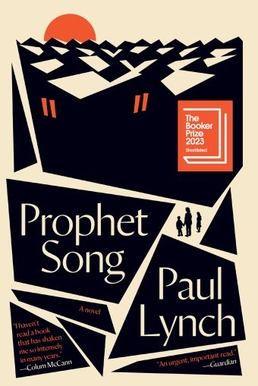
\includegraphics[height=0.5\paperheight]{images/prophet_song.jpg} &
   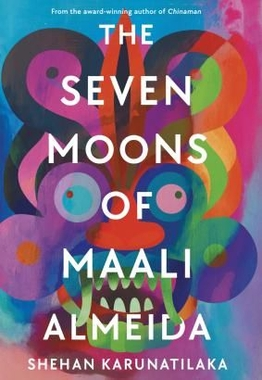
\includegraphics[height=0.5\paperheight]{images/seven_moons.png} &
   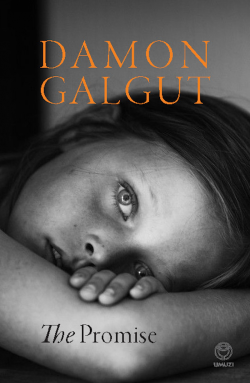
\includegraphics[height=0.5\paperheight]{images/the_promise.png}
\end{tabular}

Novels -- in fact, they are the three most recent Booker Prize winners
\end{center}

\vspace{-1em}
\blfootnote{\tiny photo credit: https://groveatlantic.com/book/prophet-song/, https://thebookerprizes.com/the-booker-library/books/the-seven-moons-of-maali-almeida, and https://www.penguinrandomhouse.co.za/book/promise/9781415210581}}}
\end{center}
\end{frame}
\begin{frame}
\begin{center}
\Large
3. What car is this?
\blfootnote{photo credit: Wikimedia Commons}
\\
\vspace{0.5em}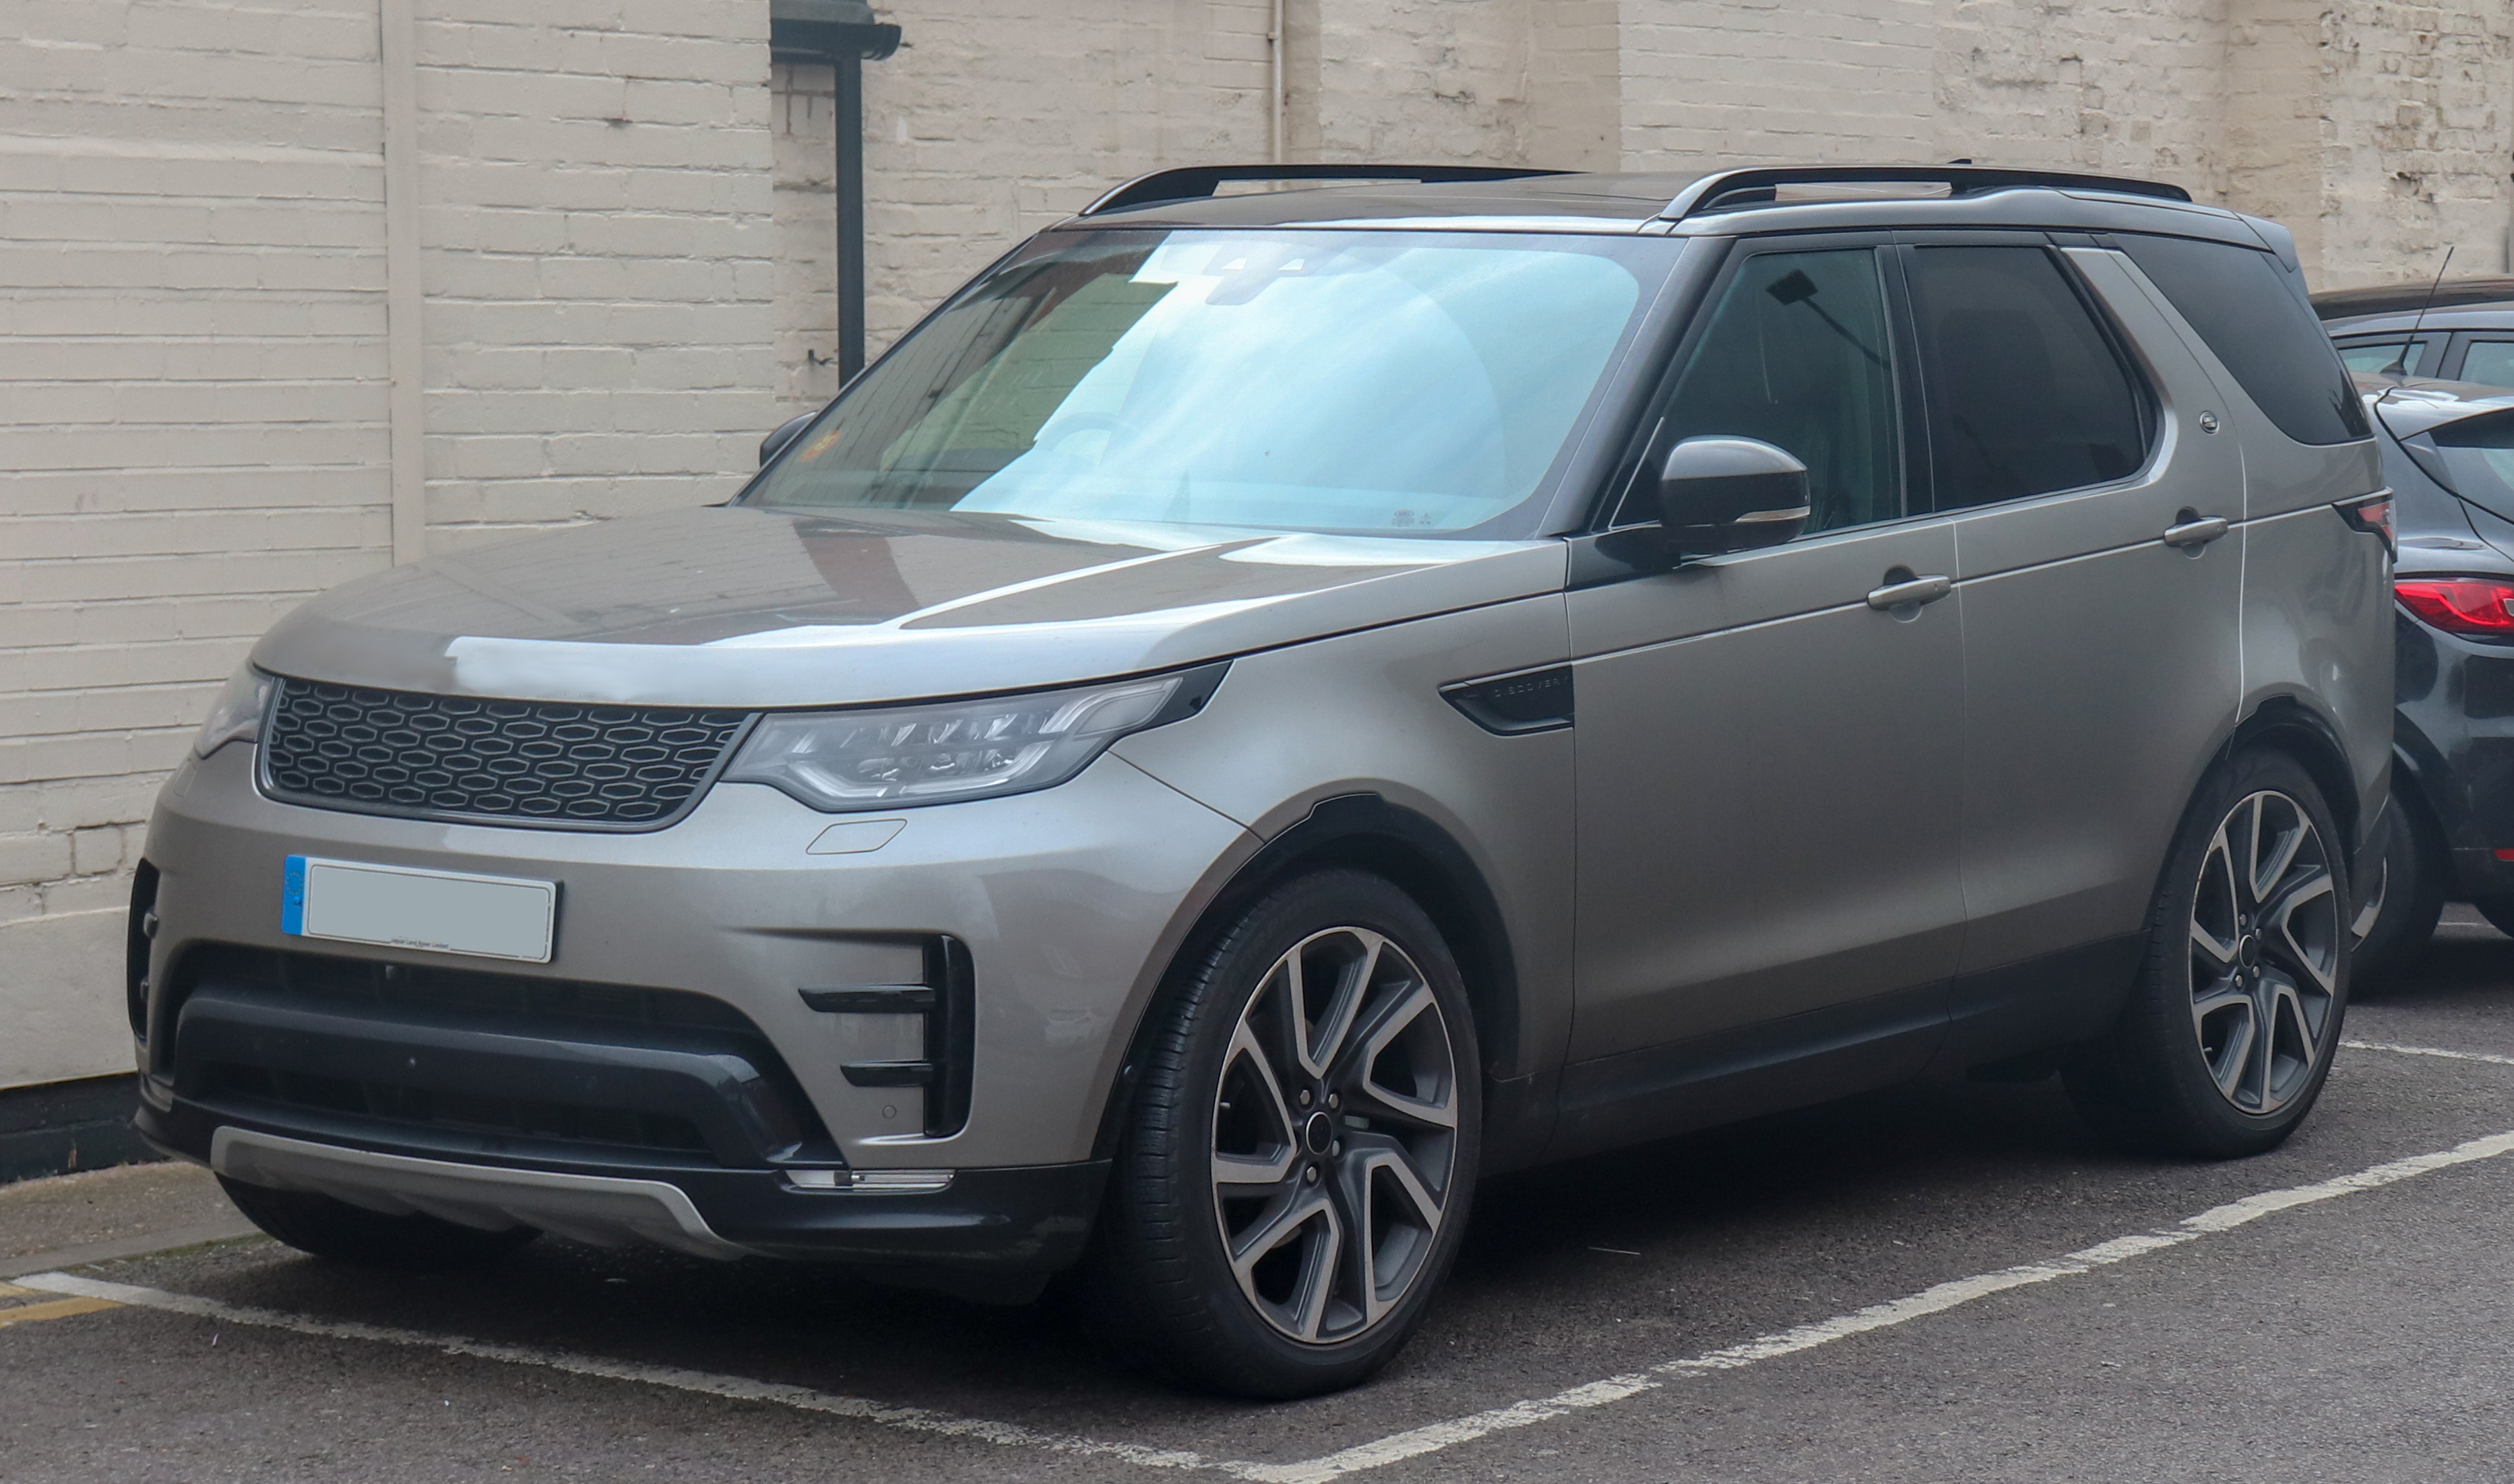
\includegraphics[height=0.6\paperheight]{images/land_rover_discovery.jpg}
\\
\onslide<2->{\vspace{1em}\textit{Land Rover Discovery}}
\end{center}
\end{frame}
\begin{frame}
\begin{center}
\Large
4. gabardine, lawn, brocade, and french terry are all examples of what?
\\
\onslide<2>{\vspace{0.5em}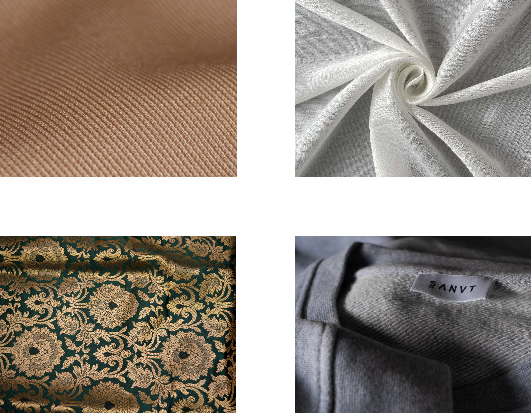
\includegraphics[height=0.6\paperheight]{images/fabrics-figure0.pdf}}
\\
\onslide<2->{\vspace{1em}\textit{fabrics}}
\end{center}
\end{frame}
\begin{frame}
\begin{center}
\Large
5. The Pritzker Prize is the most prestigious international prize in what field?
\\
\onslide<2->{\vspace{1em}\textit{Architecture}}
\end{center}
\end{frame}
\begin{frame}
\begin{center}
\Large
6. What parent company owns (among other things) DC Comics, HBO, CNN, and Eurosport?
\\
\onslide<2->{\vspace{1em}\textit{Warner Bros. Discovery}}
\end{center}
\end{frame}
\begin{frame}
\begin{center}
\Large
7. ``Die Neue Sammlung'', in Munich, is the largest what in the world? (It translates to ``The New Collection'')
\\
\onslide<2>{\vspace{0.5em}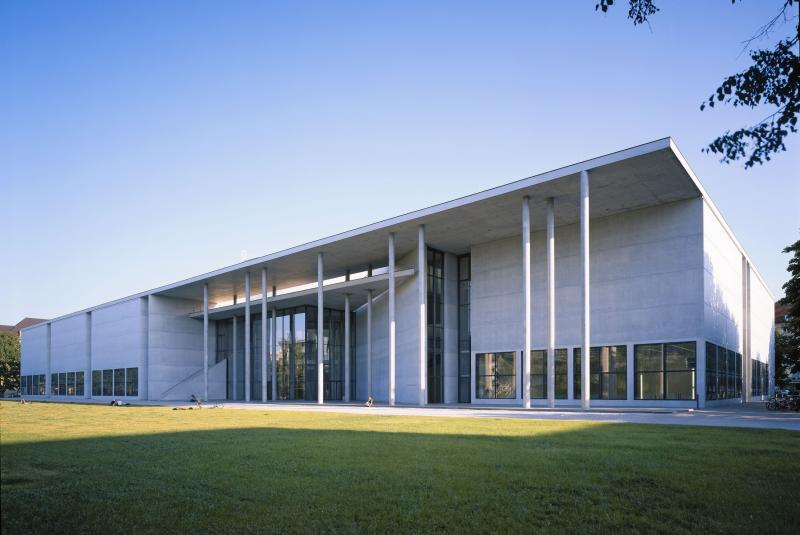
\includegraphics[height=0.6\paperheight]{images/die_neue_sammlung.jpg}}
\\
\onslide<2->{\vspace{1em}\textit{design museum}}
\end{center}
\end{frame}
\begin{frame}
\begin{center}
\Large
8. This is the opening verse to which song?
\begin{center}
    \begin{minipage}{0.6\textwidth}
        \textit{%
            Some boys kiss me \\
            Some boys hug me \\
            I think they're ok \\
            If they don't give me proper credit \\
            I just walk away}%
    \end{minipage}
\end{center}

\onslide<2->{\vspace{1em}\textit{Material Girl}}
\end{center}
\end{frame}
\begin{frame}
\begin{center}
\Huge
Round 4: Changing things up
\end{center}
\end{frame}
\begin{frame}
\begin{center}
\Large
1. What major sporting tournament is being held in Germany later this year?
\end{center}
\end{frame}
\begin{frame}
\begin{center}
\Large
2. Which 2023 TV series was widely ridiculed because it featured ghosts?
\end{center}
\end{frame}
\begin{frame}
\begin{center}
\Large
3. Which film won the 2004 Best Picture Oscar? (Spoiler alert! It was criticised by disability rights activists for its ending.)
\end{center}
\end{frame}
\begin{frame}
\begin{center}
\Large
4. The capture of Napoleon III at the Battle of Sedan marked a turning point in which war?
\end{center}
\end{frame}
\begin{frame}
\begin{center}
\Large
5. Who was Samuel Langhorne Clemens? He lived from 1835 to 1910.
\end{center}
\end{frame}
\begin{frame}
\begin{center}
\Large
6. What kind of dog is this?
\\
\vspace{0.5em}
\includegraphics[height=0.6\paperheight]{images/doge.jpg}
\end{center}
\end{frame}
\begin{frame}
\begin{center}
\Large
7. Who wrote ``Atlas Shrugged''? It is a novel that is very influential in libertarian and conservative circles, especially in America
\end{center}
\end{frame}
\begin{frame}
\begin{center}
\Large
8. What links the answers to all the questions in this round?
\end{center}
\end{frame}
\begin{frame}
\begin{center}
\Huge
Answers
\end{center}
\end{frame}
\begin{frame}
\begin{center}
\Large
1. What major sporting tournament is being held in Germany later this year?
\\
\onslide<2->{\vspace{1em}\textit{The Euros}}
\end{center}
\end{frame}
\begin{frame}
\begin{center}
\Large
2. Which 2023 TV series was widely ridiculed because it featured ghosts?
\\
\onslide<2->{\vspace{1em}\textit{The Crown}}
\end{center}
\end{frame}
\begin{frame}
\begin{center}
\Large
3. Which film won the 2004 Best Picture Oscar? (Spoiler alert! It was criticised by disability rights activists for its ending.)
\\
\onslide<2->{\vspace{1em}\textit{Million Dollar Baby}}
\end{center}
\end{frame}
\begin{frame}
\begin{center}
\Large
4. The capture of Napoleon III at the Battle of Sedan marked a turning point in which war?
\\
\onslide<2->{\vspace{1em}\textit{The Franco-Prussian War / The Franco-German War / The War of 1870}}
\end{center}
\end{frame}
\begin{frame}
\begin{center}
\Large
5. Who was Samuel Langhorne Clemens? He lived from 1835 to 1910.
\\
\onslide<2->{\vspace{1em}\textit{An author better known by his pen name: Mark Twain}}
\end{center}
\end{frame}
\begin{frame}
\begin{center}
\Large
6. What kind of dog is this?
\\
\vspace{0.5em}
\includegraphics[height=0.6\paperheight]{images/doge.jpg}
\\
\onslide<2->{\vspace{1em}\textit{a Shiba Inu}}
\end{center}
\end{frame}
\begin{frame}
\begin{center}
\Large
7. Who wrote ``Atlas Shrugged''? It is a novel that is very influential in libertarian and conservative circles, especially in America
\\
\onslide<2->{\vspace{1em}\textit{Ayn Rand}}
\end{center}
\end{frame}
\begin{frame}
\begin{center}
\Large
8. What links the answers to all the questions in this round?
\\
\onslide<2->{\vspace{1em}\textit{the \myunderline<3->{Euro}s, The \myunderline<3->{Crown}, Million \myunderline<3->{Dollar} Baby, The \myunderline<3->{Franc}o-Prussian War, \myunderline<3->{Mark} Twain, a \myunderline<3->{doge\onslide<3->{(coin)}}, Ayn \myunderline<3->{Rand}

\vspace{1em}

\onslide<4->{change}
}}
\end{center}
\end{frame}
\begin{frame}
\begin{center}
\Huge
Round 5: Numbers
\end{center}
\end{frame}
\begin{frame}
\begin{center}
\Large
1. Osmium is how many times more dense than lead? It is the densest material nautrally found on earth.
\end{center}
\end{frame}
\begin{frame}
\begin{center}
\Large
2. How many eyelids (per eye) does a polar bear have?
\end{center}
\end{frame}
\begin{frame}
\begin{center}
\Large
3. At 1200m, how many degrees below 100\textdegree C does water boil? (We are currently at 1050m.)
\end{center}
\end{frame}
\begin{frame}
\begin{center}
\Large
4. How many many Pirates of the Caribbean films are there?
\end{center}
\end{frame}
\begin{frame}
\begin{center}
\Large
5. In handball, how many players does one team have (excluding subs)?
\end{center}
\end{frame}
\begin{frame}
\begin{center}
\Large
6. Rounded to the nearest whole number, how many kilograms are there in 1 stone?
\end{center}
\end{frame}
\begin{frame}
\begin{center}
\Large
7. How many times will Halley's comet transit earth in the 21st century?
\end{center}
\end{frame}
\begin{frame}
\begin{center}
\Large
8. From takeoff to splashdown, how many days long was the Apollo 11 mission?
\end{center}
\end{frame}
\begin{frame}
\begin{center}
\Huge
Answers
\end{center}
\end{frame}
\begin{frame}
\begin{center}
\Large
1. Osmium is how many times more dense than lead? It is the densest material nautrally found on earth.
\\
\onslide<2->{\vspace{1em}\textit{2}}
\end{center}
\end{frame}
\begin{frame}
\begin{center}
\Large
2. How many eyelids (per eye) does a polar bear have?
\\
\onslide<2->{\vspace{1em}\textit{3}}
\end{center}
\end{frame}
\begin{frame}
\begin{center}
\Large
3. At 1200m, how many degrees below 100\textdegree C does water boil? (We are currently at 1050m.)
\\
\onslide<2->{\vspace{1em}\textit{4}}
\end{center}
\end{frame}
\begin{frame}
\begin{center}
\Large
4. How many many Pirates of the Caribbean films are there?
\\
\onslide<2->{\vspace{1em}\textit{5}}
\end{center}
\end{frame}
\begin{frame}
\begin{center}
\Large
5. In handball, how many players does one team have (excluding subs)?
\\
\onslide<2->{\vspace{1em}\textit{7}}
\end{center}
\end{frame}
\begin{frame}
\begin{center}
\Large
6. Rounded to the nearest whole number, how many kilograms are there in 1 stone?
\\
\onslide<2->{\vspace{1em}\textit{6}}
\end{center}
\end{frame}
\begin{frame}
\begin{center}
\Large
7. How many times will Halley's comet transit earth in the 21st century?
\\
\onslide<2->{\vspace{1em}\textit{1 (it is visible every 75 or so years, and will next appear in mid-2061)}}
\end{center}
\end{frame}
\begin{frame}
\begin{center}
\Large
8. From takeoff to splashdown, how many days long was the Apollo 11 mission?
\\
\onslide<2->{\vspace{1em}\textit{8}}
\end{center}
\end{frame}
\begin{frame}
\begin{center}
\Huge
Pictures: Surmise by size
\end{center}
\end{frame}
\begin{frame}
\begin{center}
\Large
1. 
\\
\vspace{0.5em}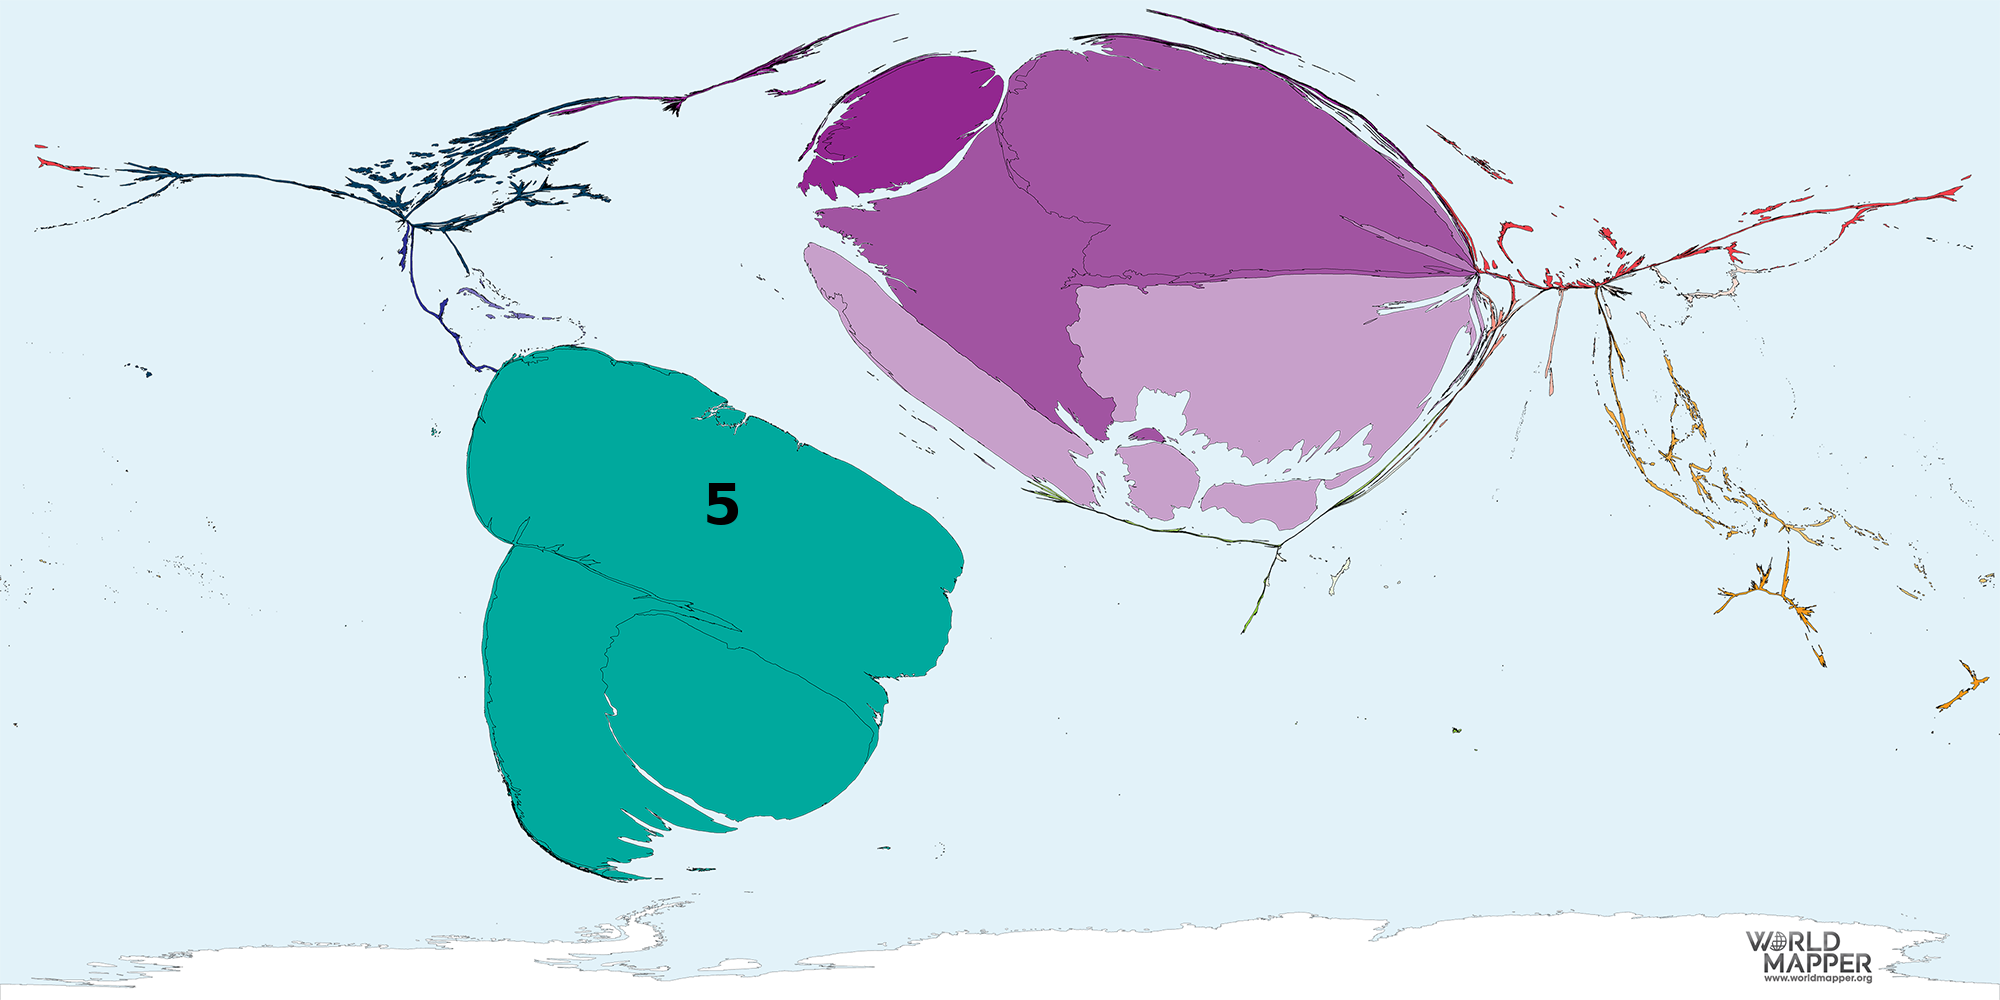
\includegraphics[height=0.6\paperheight]{maps/picture_1.png}
\\
\onslide<2->{\vspace{1em}\textit{FIFA World Cup wins}}
\end{center}
\end{frame}
\begin{frame}
\begin{center}
\Large
2. 
\\
\vspace{0.5em}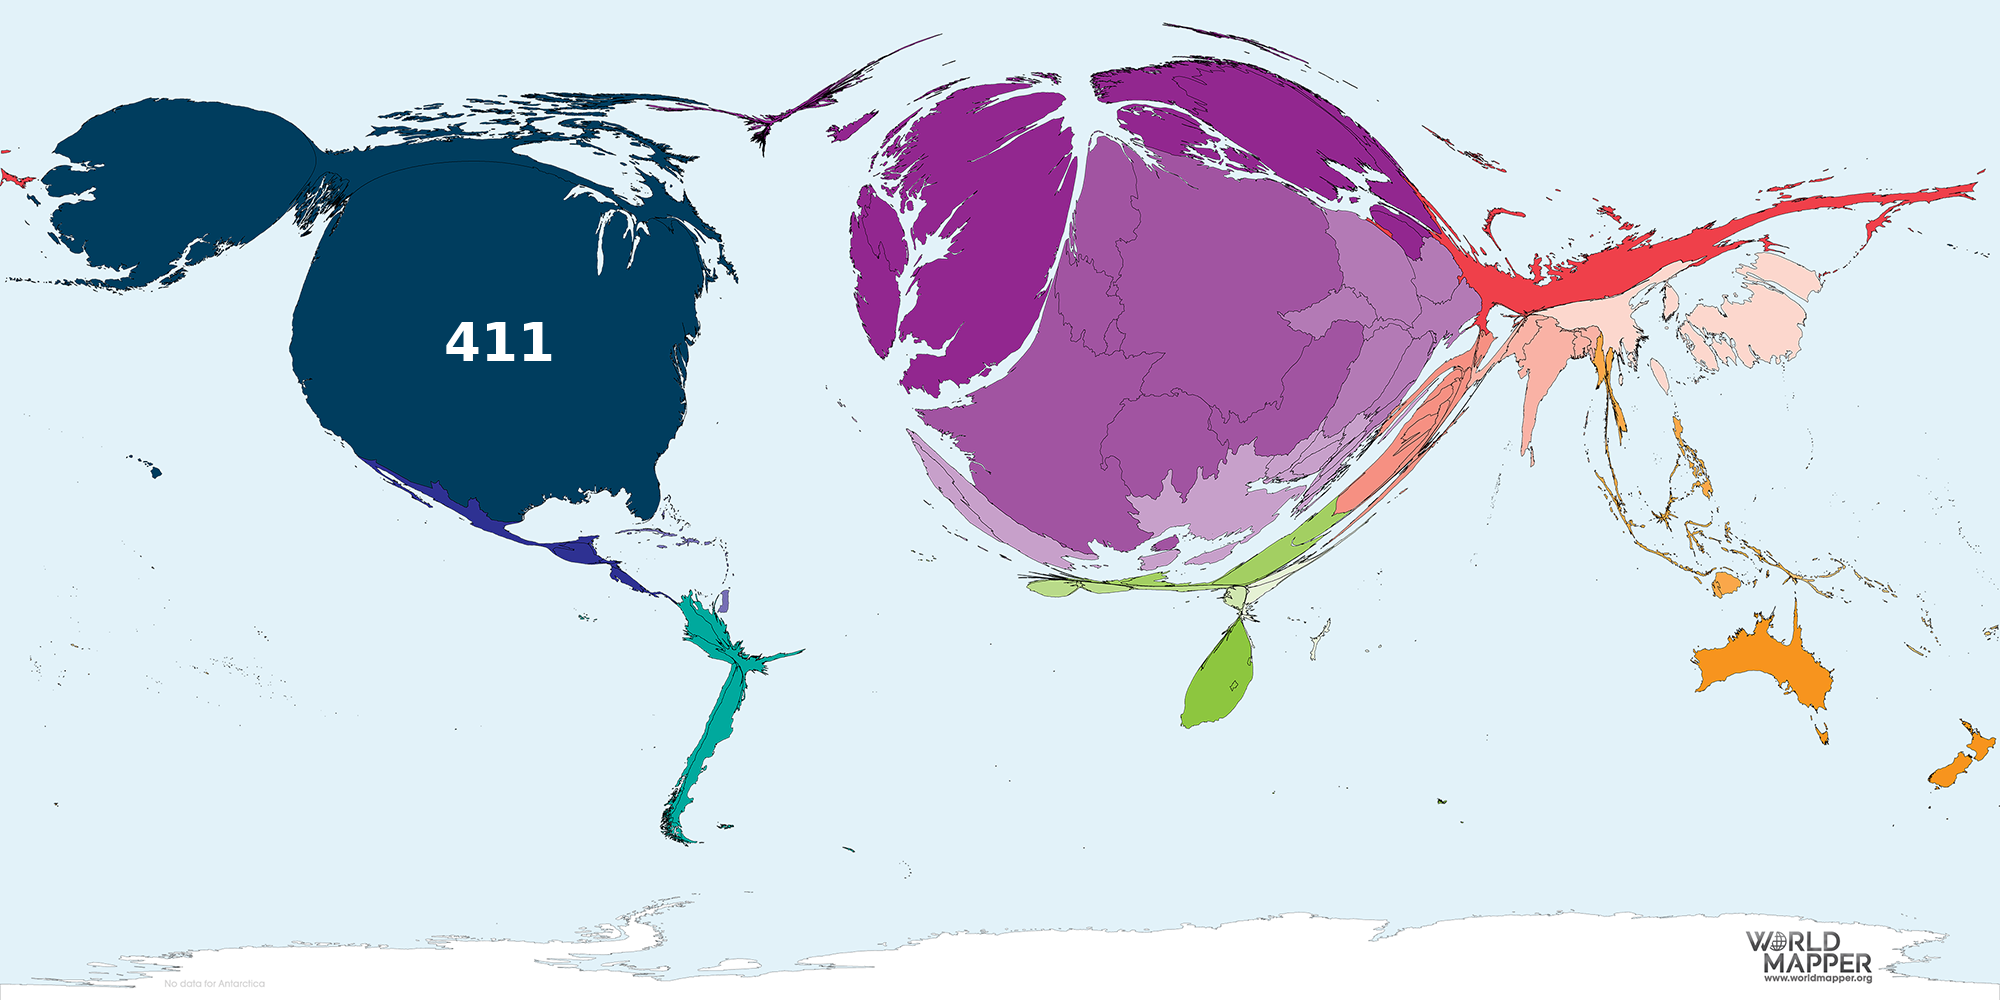
\includegraphics[height=0.6\paperheight]{maps/picture_2.png}
\\
\onslide<2->{\vspace{1em}\textit{Nobel laureates}}
\end{center}
\end{frame}
\begin{frame}
\begin{center}
\Large
3. 
\\
\vspace{0.5em}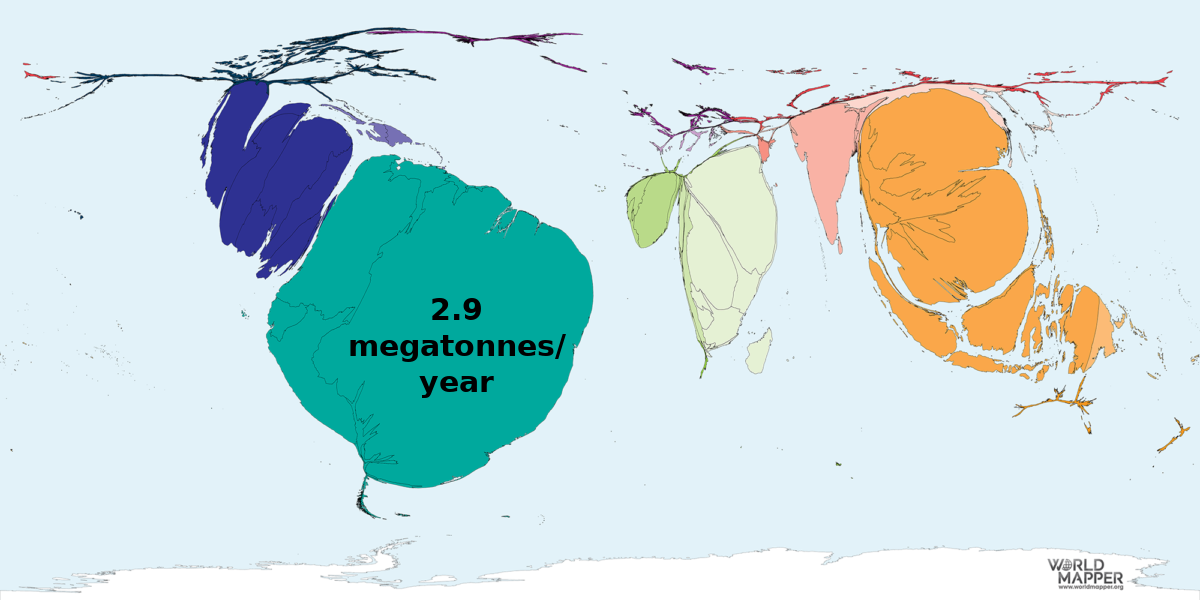
\includegraphics[height=0.6\paperheight]{maps/picture_3.png}
\\
\onslide<2->{\vspace{1em}\textit{coffee production}}
\end{center}
\end{frame}
\begin{frame}
\begin{center}
\Large
4. 
\\
\vspace{0.5em}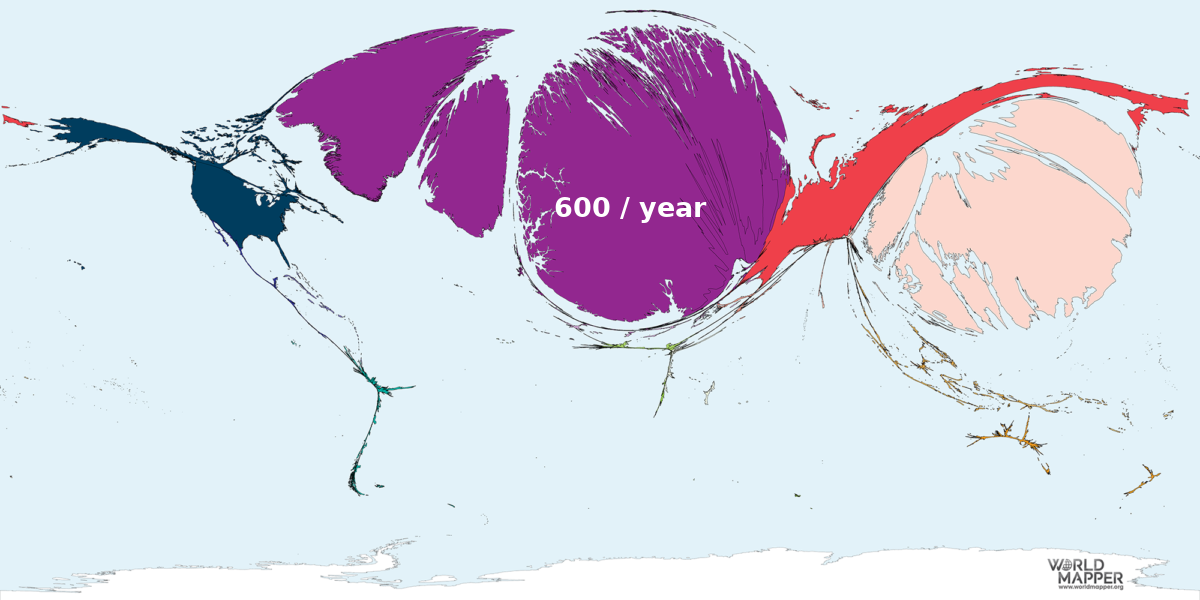
\includegraphics[height=0.6\paperheight]{maps/picture_4.png}
\\
\onslide<2->{\vspace{1em}\textit{whales killed}}
\end{center}
\end{frame}
\begin{frame}
\begin{center}
\Large
5. 
\\
\vspace{0.5em}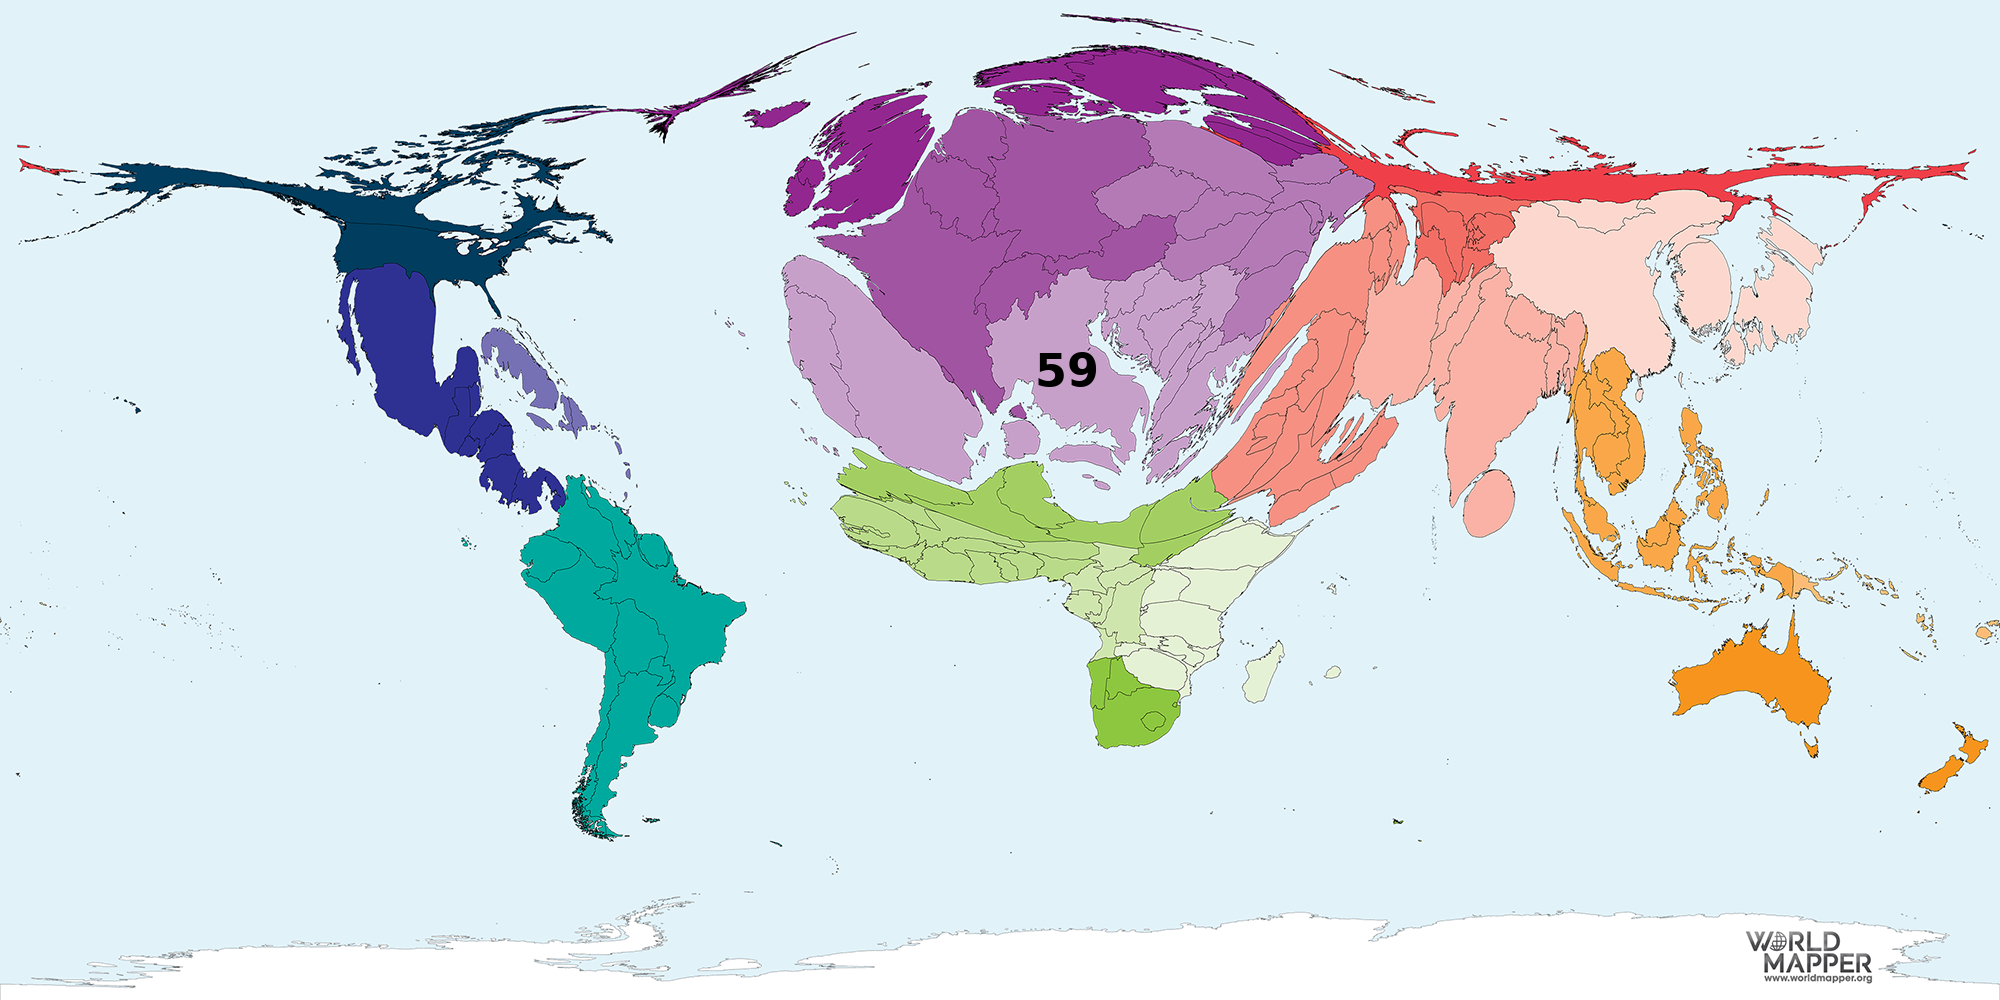
\includegraphics[height=0.6\paperheight]{maps/picture_5.png}
\\
\onslide<2->{\vspace{1em}\textit{UNESCO world heritage sites}}
\end{center}
\end{frame}
\begin{frame}
\begin{center}
\Large
6. 
\\
\vspace{0.5em}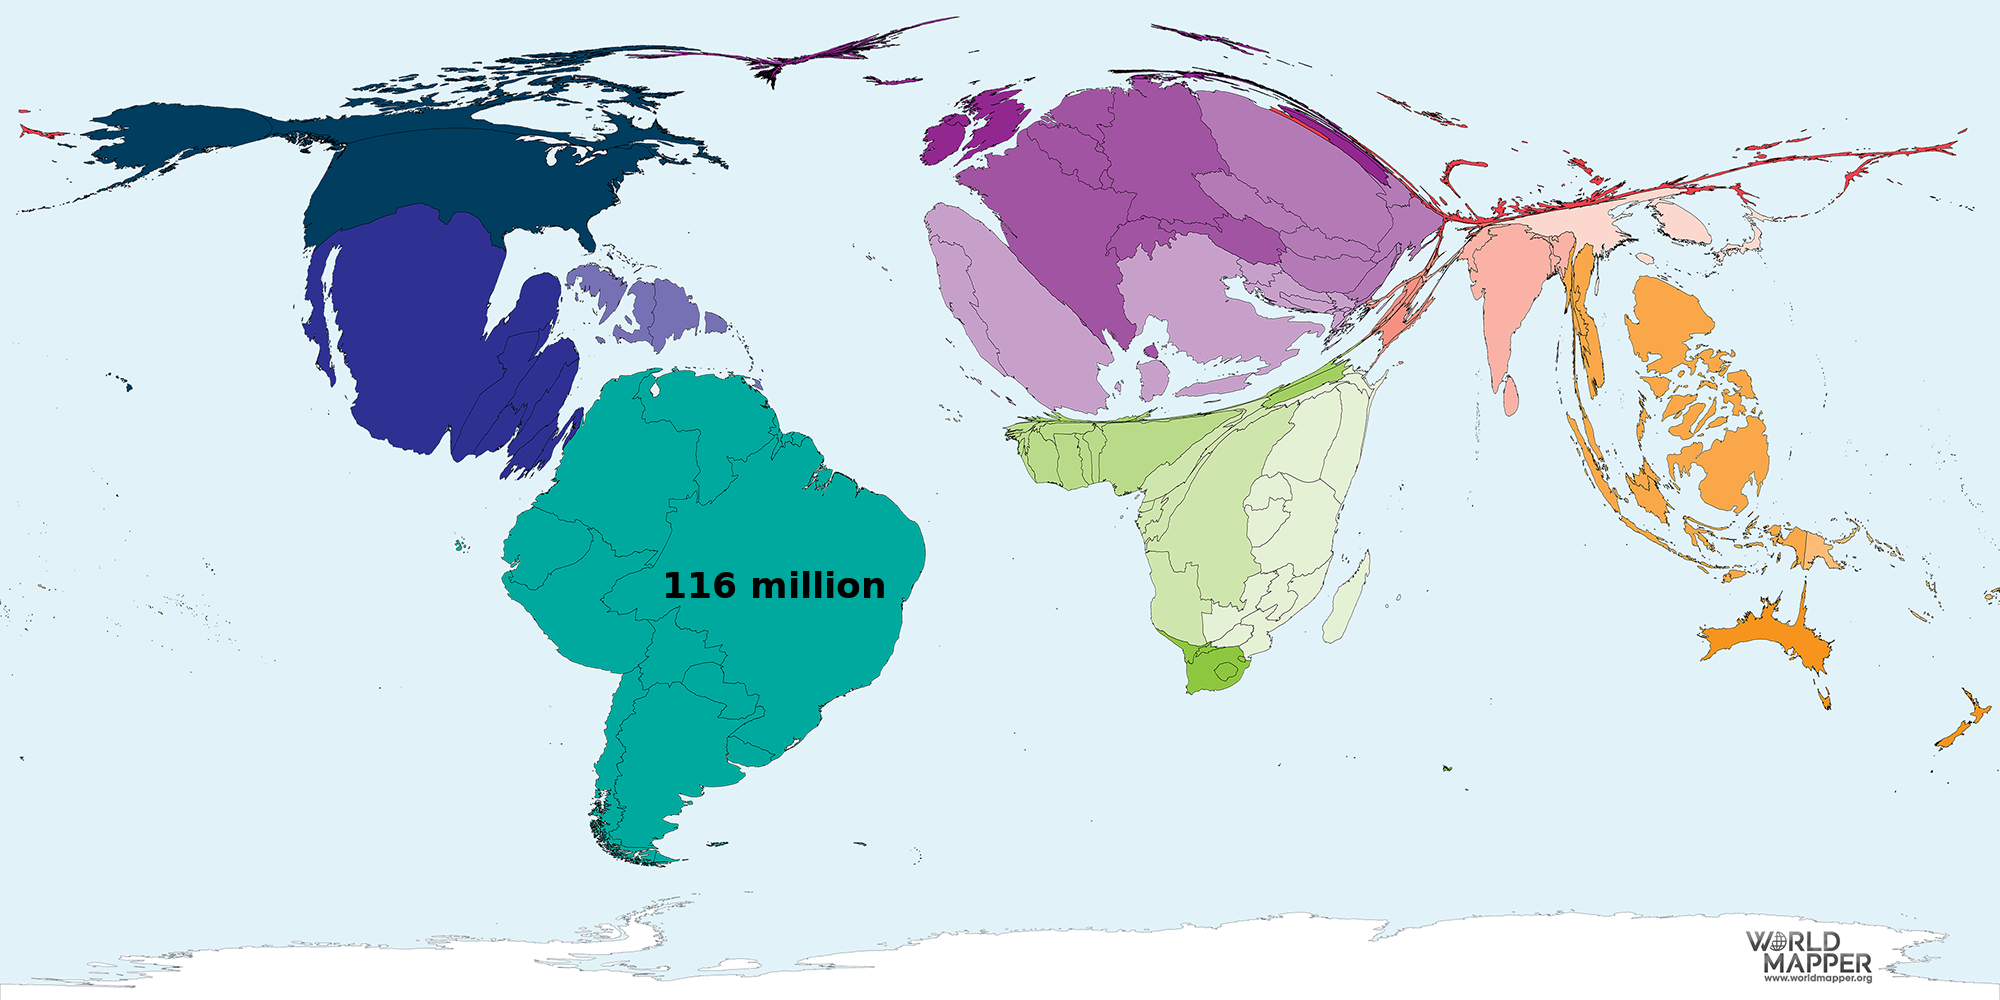
\includegraphics[height=0.6\paperheight]{maps/picture_6.png}
\\
\onslide<2->{\vspace{1em}\textit{Catholics}}
\end{center}
\end{frame}
\begin{frame}
\begin{center}
\Large
7. 
\\
\vspace{0.5em}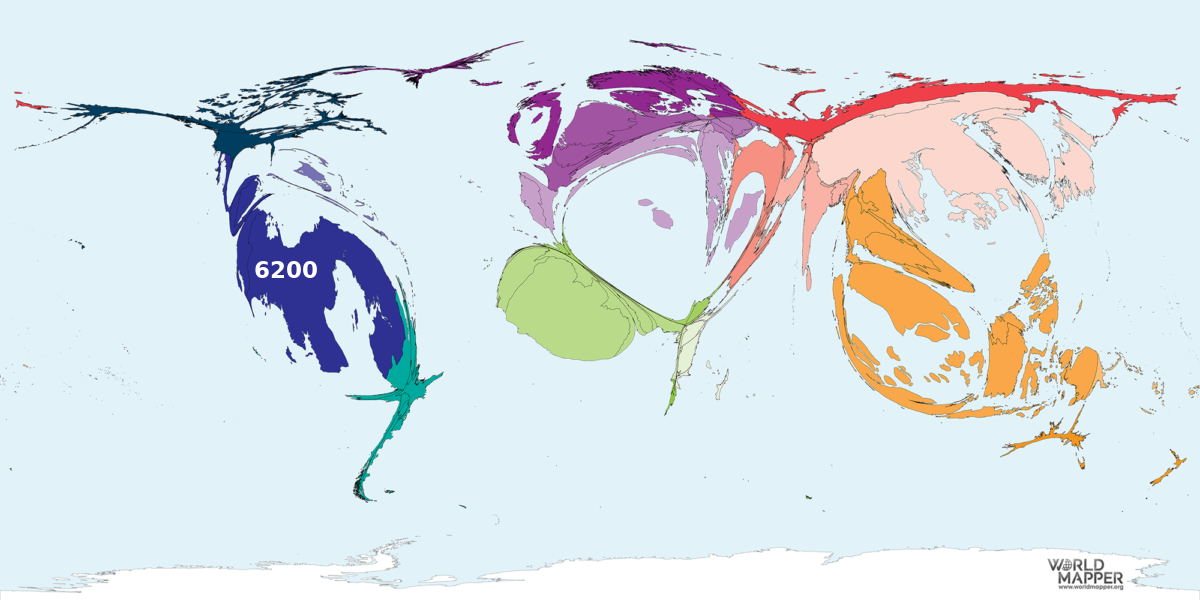
\includegraphics[height=0.6\paperheight]{maps/picture_7.png}
\\
\onslide<2->{\vspace{1em}\textit{registered ships}}
\end{center}
\end{frame}
\begin{frame}
\begin{center}
\Large
8. 
\\
\vspace{0.5em}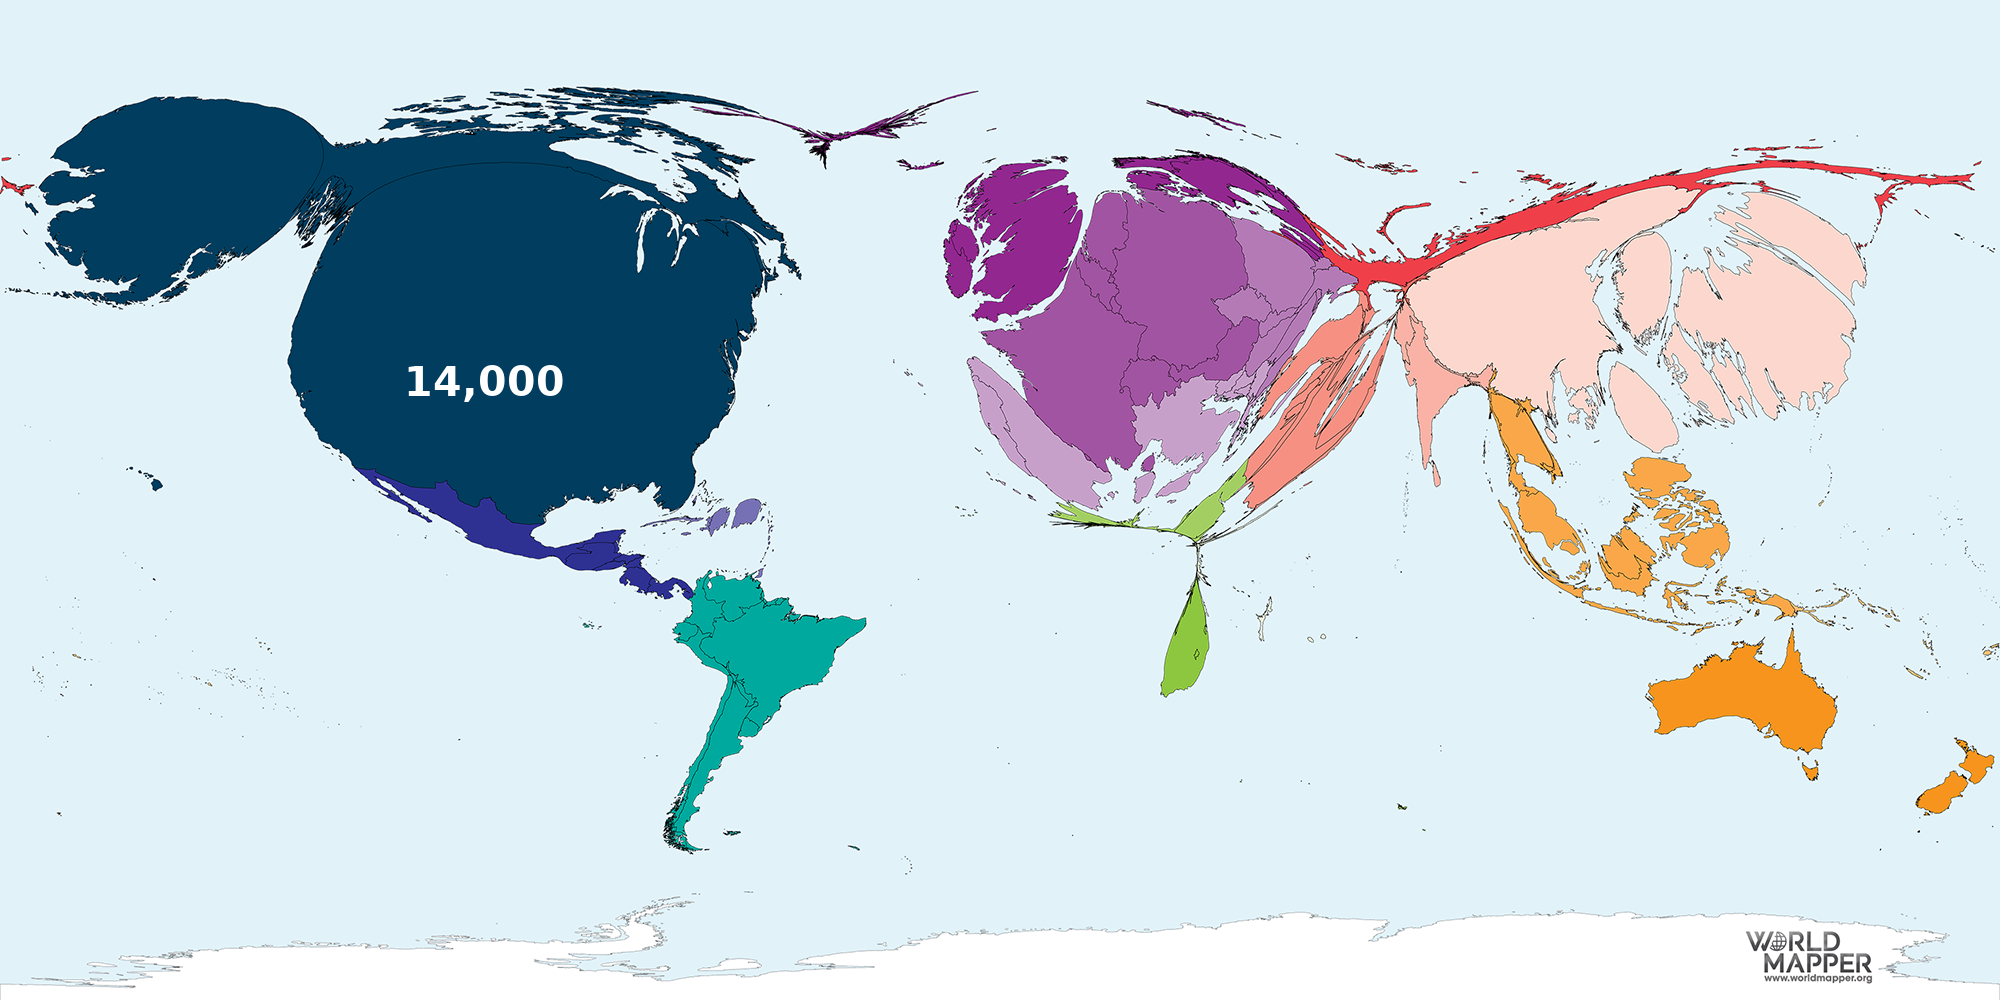
\includegraphics[height=0.6\paperheight]{maps/picture_8.png}
\\
\onslide<2->{\vspace{1em}\textit{McDonalds}}
\end{center}
\end{frame}
\begin{frame}
\begin{center}
\Huge
Puzzles: Connect Four
\end{center}
\end{frame}
\begin{frame}
\begin{center}
\Large
1. \leavevmode \\
\begin{center}
    \begin{minipage}{0.6\textwidth}
        \textit{%
            sharp taste \\
            words set to music \\
            Solo character \\
            archenemy of Flash Gordon}%
    \end{minipage}
\end{center}

\onslide<2->{\vspace{1em}\textit{Tang, Song, Han, and Ming: all Chinese dynasties}}
\end{center}
\end{frame}
\begin{frame}
\begin{center}
    \Large 2.
    \vspace{1em}

    \begin{minipage}{0.8\textwidth}
        \textit{%
		test: objection   \only<3->{= \textbf{pro}test }and competition \only<3->{= \textbf{con}test}\\
            found: deep   \only<4->{= \textbf{pro}found }and confuse     \only<4->{= \textbf{con}found}\\
            tract: extend \only<5->{= \textbf{pro}tract }and agreement   \only<5->{= \textbf{con}tract}\\
            duct: goods   \only<6->{= \textbf{pro}duct }and behaviour   \only<6->{= \textbf{con}duct}}%
    \end{minipage}
    \vspace{1em}

    \onslide<2->{It's a pros and cons list!}
\end{center}

\end{frame}
\begin{frame}
\begin{center}
\Large
3. \leavevmode \\
\begin{center}
\setchessboard{boardfontsize=8pt, labelleft=false, labelbottom=false} % , labelfontsize=6pt
\newgame
\chessboard[setfen=4K3/8/8/8/8/8/8/8 w - - 0 0,showmover=False]
\chessboard[setfen=8/8/6K1/8/8/8/8/8 w - - 0 0,showmover=False]
\chessboard[setfen=8/8/8/8/8/8/4Q3/8 w - - 0 0,showmover=False]
\chessboard[setfen=8/8/8/8/8/2K5/8/8 w - - 0 0,showmover=False]
\end{center}
\onslide<2->{\vspace{1em}\textit{Ke8, Kg6, Qe2, and Kc3: British monarchs (Edward VIII, George VI, Elizabeth II, and Charles III)}}
\end{center}
\end{frame}
\begin{frame}
\begin{center}
\Large
4. \leavevmode \\
\begin{center}
    \begin{minipage}{0.6\textwidth}
        \textit{%
            Somalia: very bad \\
            Syria: bad \\
            Philippines: average \\
            New Zealand: good}%
    \end{minipage}
\end{center}

\onslide<2->{\vspace{1em}\textit{\onslide<2->{Time to review some flags!}

\vspace{1em}

\begin{tabular}{cccc}
      \onslide<2->{
\includegraphics[height=0.2\paperheight]{images/flag_somalia.png}} &
      \onslide<4->{
\includegraphics[height=0.2\paperheight]{images/flag_syria.png}} &
      \onslide<6->{
\includegraphics[height=0.2\paperheight]{images/flag_philippines.png}} &
      \onslide<8->{
\includegraphics[height=0.2\paperheight]{images/flag_nz.png}} \\
      \onslide<3->{$\bigstar\textcolor{lightgrey}{\bigstar\bigstar\bigstar\bigstar}$} &
      \onslide<5->{$\bigstar\bigstar\textcolor{lightgrey}{\bigstar\bigstar\bigstar}$} &
      \onslide<7->{$\bigstar\bigstar\bigstar\textcolor{lightgrey}{\bigstar\bigstar}$} &
      \onslide<9->{$\bigstar\bigstar\bigstar\bigstar\textcolor{lightgrey}{\bigstar}$}
\end{tabular}}}
\end{center}
\end{frame}
\end{document}